\documentclass[twoside]{book}

% Packages required by doxygen
\usepackage{fixltx2e}
\usepackage{calc}
\usepackage{doxygen}
\usepackage[export]{adjustbox} % also loads graphicx
\usepackage{graphicx}
\usepackage[utf8]{inputenc}
\usepackage{makeidx}
\usepackage{multicol}
\usepackage{multirow}
\PassOptionsToPackage{warn}{textcomp}
\usepackage{textcomp}
\usepackage[nointegrals]{wasysym}
\usepackage[table]{xcolor}

% Font selection
\usepackage[T1]{fontenc}
\usepackage[scaled=.90]{helvet}
\usepackage{courier}
\usepackage{amssymb}
\usepackage{sectsty}
\renewcommand{\familydefault}{\sfdefault}
\allsectionsfont{%
  \fontseries{bc}\selectfont%
  \color{darkgray}%
}
\renewcommand{\DoxyLabelFont}{%
  \fontseries{bc}\selectfont%
  \color{darkgray}%
}
\newcommand{\+}{\discretionary{\mbox{\scriptsize$\hookleftarrow$}}{}{}}

% Page & text layout
\usepackage{geometry}
\geometry{%
  a4paper,%
  top=2.5cm,%
  bottom=2.5cm,%
  left=2.5cm,%
  right=2.5cm%
}
\tolerance=750
\hfuzz=15pt
\hbadness=750
\setlength{\emergencystretch}{15pt}
\setlength{\parindent}{0cm}
\setlength{\parskip}{3ex plus 2ex minus 2ex}
\makeatletter
\renewcommand{\paragraph}{%
  \@startsection{paragraph}{4}{0ex}{-1.0ex}{1.0ex}{%
    \normalfont\normalsize\bfseries\SS@parafont%
  }%
}
\renewcommand{\subparagraph}{%
  \@startsection{subparagraph}{5}{0ex}{-1.0ex}{1.0ex}{%
    \normalfont\normalsize\bfseries\SS@subparafont%
  }%
}
\makeatother

% Headers & footers
\usepackage{fancyhdr}
\pagestyle{fancyplain}
\fancyhead[LE]{\fancyplain{}{\bfseries\thepage}}
\fancyhead[CE]{\fancyplain{}{}}
\fancyhead[RE]{\fancyplain{}{\bfseries\leftmark}}
\fancyhead[LO]{\fancyplain{}{\bfseries\rightmark}}
\fancyhead[CO]{\fancyplain{}{}}
\fancyhead[RO]{\fancyplain{}{\bfseries\thepage}}
\fancyfoot[LE]{\fancyplain{}{}}
\fancyfoot[CE]{\fancyplain{}{}}
\fancyfoot[RE]{\fancyplain{}{\bfseries\scriptsize Generated by Doxygen }}
\fancyfoot[LO]{\fancyplain{}{\bfseries\scriptsize Generated by Doxygen }}
\fancyfoot[CO]{\fancyplain{}{}}
\fancyfoot[RO]{\fancyplain{}{}}
\renewcommand{\footrulewidth}{0.4pt}
\renewcommand{\chaptermark}[1]{%
  \markboth{#1}{}%
}
\renewcommand{\sectionmark}[1]{%
  \markright{\thesection\ #1}%
}

% Indices & bibliography
\usepackage{natbib}
\usepackage[titles]{tocloft}
\setcounter{tocdepth}{3}
\setcounter{secnumdepth}{5}
\makeindex

% Hyperlinks (required, but should be loaded last)
\usepackage{ifpdf}
\ifpdf
  \usepackage[pdftex,pagebackref=true]{hyperref}
\else
  \usepackage[ps2pdf,pagebackref=true]{hyperref}
\fi
\hypersetup{%
  colorlinks=true,%
  linkcolor=blue,%
  citecolor=blue,%
  unicode%
}

% Custom commands
\newcommand{\clearemptydoublepage}{%
  \newpage{\pagestyle{empty}\cleardoublepage}%
}

\usepackage{caption}
\captionsetup{labelsep=space,justification=centering,font={bf},singlelinecheck=off,skip=4pt,position=top}

%===== C O N T E N T S =====

\begin{document}

% Titlepage & ToC
\hypersetup{pageanchor=false,
             bookmarksnumbered=true,
             pdfencoding=unicode
            }
\pagenumbering{alph}
\begin{titlepage}
\vspace*{7cm}
\begin{center}%
{\Large Enigma }\\
\vspace*{1cm}
{\large Generated by Doxygen 1.8.14}\\
\end{center}
\end{titlepage}
\clearemptydoublepage
\pagenumbering{roman}
\tableofcontents
\clearemptydoublepage
\pagenumbering{arabic}
\hypersetup{pageanchor=true}

%--- Begin generated contents ---
\chapter{R\+E\+A\+D\+ME}
\label{md__home_ravib_catkin_ws_src_enigma__r_e_a_d_m_e}
\Hypertarget{md__home_ravib_catkin_ws_src_enigma__r_e_a_d_m_e}
\href{https://travis-ci.org/raviBhadeshiya/enigma}{\tt } \mbox{[}\mbox{]}(L\+I\+C\+E\+N\+SE) \section*{enigma}

One of the big tech topics of 2017 is automation−whether and how robots can replace or augmentwork done by humans. In order to do the kind of work a human security guard would normally do,the robot should use cameras, sensors, navigation equipment, and electric motors−all packed intoits dome-\/shaped body with a big rechargeable battery and a computer. The autonomous guidancesystem allows the robot to store its cruise route and move automatically without an operator. It is based on the input video camera and other sensors; allowing the U\+GV to follow the path accurately,detect and avoid the obstacles. The package present real time indoor security device we call Enigma! The robotics system using Turtl\+Bot to perform a surveillance of a virtual environment generated by 3D Gazebo simulator. This system performs an indoor surveillance byperforming S\+L\+AM and video processing, in order to ensure that any possible ananomly is detected by the color of an object such as Red or Green colored cylinder.

The system will 3\+D-\/map an unknown environment. While 3\+D-\/mapping the unknown environment, the bot will perform patrol by running the detection node to find the ananomly such as red-\/colored cylinder object. There is be custom world with red and green colored cylinders. The detection algorithm is very naive such as transform image to H\+SV space, then thresholding and region detection for the object (red colored cylinder).Then object count is publish on the \char`\"{}\textbackslash{}detection\char`\"{} topic and user will get notified by info message. Please check below\+:



\subparagraph*{Output with 3\+D-\/mapping}



\subsection*{Dependency}


\begin{DoxyItemize}
\item \href{http://wiki.ros.org/ROS/Installation}{\tt R\+OS Kinetic} on Ubuntu 16.\+04
\item \href{http://gazebosim.org/}{\tt Gazebo}
\item \href{http://wiki.ros.org/Robots/TurtleBot}{\tt Turtle\+Bot}
\item \href{http://wiki.ros.org/octomap}{\tt octomap}
\end{DoxyItemize}

\#\# Standard install via command-\/line 
\begin{DoxyCode}
$ mkdir -p ~/catkin\_ws/src
$ cd ~/catkin\_ws/
$ catkin\_make
$ source devel/setup.bash
$ cd src/
$ git clone --recursive https://github.com/raviBhadeshiya/enigma.git
$ cd ..
$ catkin\_make
\end{DoxyCode}
 $>$N\+O\+TE\+: Missing dependency can be added via following command but highly encourage to install sepratly!


\begin{DoxyCode}
~/catkin\_ws$ rosdep install --from-paths src --ignore-src --rosdistro kinetic -y
\end{DoxyCode}
 However for octomap installation follow the tutorial\+:\href{http://wiki.ros.org/octomap}{\tt link} 

 \subsection*{Execution}

The following package can ber start with single launch file as follows\+: 
\begin{DoxyCode}
$ roslaunch enigma enigma.launch
\end{DoxyCode}
 $>$Arguments\+: record\+:=true for recording rosbag file and world\+:=enigma/map/final\+\_\+world\+\_\+1 for testing custom word file.

$>$Note\+: roslaunch will automatically start roscore if it detects that it is not already running. \subparagraph*{Package Interface\+:}

The following package use the rosservice to intract with package. \subparagraph*{Start/\+Stop Robot Motion}

To call this service, open a new terminal and type\+:


\begin{DoxyCode}
$ rosservice call /robotSwitch true
\end{DoxyCode}
 Argument true will cause robot to start motion and false will cause robot to stop the motion. $>$Note\+: After roslaunch if robot is not moving, call this service to start motion. \subparagraph*{Change Robot Speed}

If you want to change the speed of the robot,then open a new terminal and make new service call\+:


\begin{DoxyCode}
$ rosservice call /robotSpeed 0.8
\end{DoxyCode}
 Argument will set the robot max speed to 0.\+8 but you can pass any valid speed between 0 to 1.\+0 \subparagraph*{Start/\+Stop \hyperlink{class_detection}{Detection}}

To call this service, similarly open a new terminal and type\+: 
\begin{DoxyCode}
$ rosservice call /detectionSwitch true
\end{DoxyCode}
 Argument true will cause detection to start detection and false will cause to stop. If \hyperlink{class_detection}{Detection} topic is not being publishe, then call this service to start detection. \subparagraph*{Saving the Octomap}

The octomap\+\_\+server loads a 3D map (as Octree-\/based Octo\+Map) and distributes it to other nodes in a compact binary format. It also allows to incrementally build 3D Octo\+Maps, and provides map saving in the node octomap\+\_\+saver. 
\begin{DoxyCode}
$ rosrun octomap\_server octopmap\_saver -f enigma\_map.ot
\end{DoxyCode}


\paragraph*{Running the node separately}

$>$Caution\+: Make sure turtlebot-\/gazebo is running.

Running nodes requires you have a R\+OS core started. A R\+OS core is a collection of nodes and programs that are pre-\/requisites of a R\+O\+S-\/based system. You must have a roscore running in order for R\+OS nodes to communicate. Open a new shell, and type\+: 
\begin{DoxyCode}
$ roscore
\end{DoxyCode}
 \subparagraph*{Node}

The \hyperlink{class_enigma}{Enigma} node can be run by opening new shell, and type\+: 
\begin{DoxyCode}
$ rosrun enigma enigma\_node
\end{DoxyCode}
 and for detection node can be run by opening new shell, and type\+: 
\begin{DoxyCode}
$ rosrun enigma detection\_node
\end{DoxyCode}
 

 \subsection*{Testing}

There are two main unit tests in this module\+:testing for enigma and detection. To run all testcase of this module\+: 
\begin{DoxyCode}
$ cd catkin\_ws
$ catkin\_make run\_tests
\end{DoxyCode}
 Or using rostest, type this command in new terminal\+: 
\begin{DoxyCode}
$ rostest enigma enigma\_check.test
$ rostest enigma detection\_check.test
\end{DoxyCode}
 

 \subsubsection*{Solo Iterative Process}

Solo Iterative process was used for developing this package and it can be observed that estimates were improved over time. For detailed spreadsheet\+: \href{https://docs.google.com/spreadsheets/d/10tGs0astZB6bFPMXlLJwByrlTDJi1ZNfbLnQGZDo5Xo/edit?usp=sharing}{\tt }

For sprint planning\+: \href{https://docs.google.com/document/d/1hJ8q-_5HhWBHmOfXV9d_nZg0-gOeu8520EBP83TKBbI/edit?usp=sharing}{\tt Click Here}

\subsubsection*{Presentation}

Slides \+: \href{https://docs.google.com/presentation/d/1KM6IbHGB0xqtuu0a0-CgijcBst5EShQxvior-kgVUcg/edit?usp=sharing}{\tt click here} 
\chapter{Class Index}
\section{Class List}
Here are the classes, structs, unions and interfaces with brief descriptions\+:\begin{DoxyCompactList}
\item\contentsline{section}{\hyperlink{class_detection}{Detection} \\*Class for detection }{\pageref{class_detection}}{}
\item\contentsline{section}{\hyperlink{class_enigma}{Enigma} \\*Class for enigma for robot behavior }{\pageref{class_enigma}}{}
\item\contentsline{section}{\hyperlink{struct_test_helper}{Test\+Helper} \\*Struct for service callback helper }{\pageref{struct_test_helper}}{}
\end{DoxyCompactList}

\chapter{File Index}
\section{File List}
Here is a list of all documented files with brief descriptions\+:\begin{DoxyCompactList}
\item\contentsline{section}{/home/ravib/catkin\+\_\+ws/src/enigma/doc/html/{\bfseries \+\_\+detection\+\_\+test\+\_\+8cpp.\+js} }{\pageref{__detection__test__8cpp_8js}}{}
\item\contentsline{section}{/home/ravib/catkin\+\_\+ws/src/enigma/doc/html/{\bfseries \+\_\+enigma\+\_\+test\+\_\+8cpp.\+js} }{\pageref{__enigma__test__8cpp_8js}}{}
\item\contentsline{section}{/home/ravib/catkin\+\_\+ws/src/enigma/doc/html/{\bfseries annotated\+\_\+dup.\+js} }{\pageref{annotated__dup_8js}}{}
\item\contentsline{section}{/home/ravib/catkin\+\_\+ws/src/enigma/doc/html/{\bfseries class\+\_\+detection.\+js} }{\pageref{class__detection_8js}}{}
\item\contentsline{section}{/home/ravib/catkin\+\_\+ws/src/enigma/doc/html/{\bfseries class\+\_\+enigma.\+js} }{\pageref{class__enigma_8js}}{}
\item\contentsline{section}{/home/ravib/catkin\+\_\+ws/src/enigma/doc/html/{\bfseries dir\+\_\+2f4b7a607ea055218aab4b7ed1e45e78.\+js} }{\pageref{dir__2f4b7a607ea055218aab4b7ed1e45e78_8js}}{}
\item\contentsline{section}{/home/ravib/catkin\+\_\+ws/src/enigma/doc/html/{\bfseries dir\+\_\+3e6cb690d24cf9d8c1433757d95948c3.\+js} }{\pageref{dir__3e6cb690d24cf9d8c1433757d95948c3_8js}}{}
\item\contentsline{section}{/home/ravib/catkin\+\_\+ws/src/enigma/doc/html/{\bfseries dir\+\_\+58ce381989b3e407ff7c195a9fac118a.\+js} }{\pageref{dir__58ce381989b3e407ff7c195a9fac118a_8js}}{}
\item\contentsline{section}{/home/ravib/catkin\+\_\+ws/src/enigma/doc/html/{\bfseries dir\+\_\+5c9b1b03f6e45e6a48c8e8f7b0f905ad.\+js} }{\pageref{dir__5c9b1b03f6e45e6a48c8e8f7b0f905ad_8js}}{}
\item\contentsline{section}{/home/ravib/catkin\+\_\+ws/src/enigma/doc/html/{\bfseries dir\+\_\+7c859f3878cb32062c29919224ce2290.\+js} }{\pageref{dir__7c859f3878cb32062c29919224ce2290_8js}}{}
\item\contentsline{section}{/home/ravib/catkin\+\_\+ws/src/enigma/doc/html/{\bfseries dir\+\_\+c611425d629fc70798438c4e0f69031b.\+js} }{\pageref{dir__c611425d629fc70798438c4e0f69031b_8js}}{}
\item\contentsline{section}{/home/ravib/catkin\+\_\+ws/src/enigma/doc/html/{\bfseries dir\+\_\+d4e96c0a55d689de9c667dda1b4fd25e.\+js} }{\pageref{dir__d4e96c0a55d689de9c667dda1b4fd25e_8js}}{}
\item\contentsline{section}{/home/ravib/catkin\+\_\+ws/src/enigma/doc/html/{\bfseries dynsections.\+js} }{\pageref{dynsections_8js}}{}
\item\contentsline{section}{/home/ravib/catkin\+\_\+ws/src/enigma/doc/html/{\bfseries enigma\+\_\+\+\_\+node\+\_\+8cpp.\+js} }{\pageref{enigma____node__8cpp_8js}}{}
\item\contentsline{section}{/home/ravib/catkin\+\_\+ws/src/enigma/doc/html/{\bfseries enigma\+\_\+\+\_\+test\+\_\+\+\_\+node\+\_\+8cpp.\+js} }{\pageref{enigma____test____node__8cpp_8js}}{}
\item\contentsline{section}{/home/ravib/catkin\+\_\+ws/src/enigma/doc/html/{\bfseries files\+\_\+dup.\+js} }{\pageref{files__dup_8js}}{}
\item\contentsline{section}{/home/ravib/catkin\+\_\+ws/src/enigma/doc/html/{\bfseries jquery.\+js} }{\pageref{jquery_8js}}{}
\item\contentsline{section}{/home/ravib/catkin\+\_\+ws/src/enigma/doc/html/{\bfseries menu.\+js} }{\pageref{menu_8js}}{}
\item\contentsline{section}{/home/ravib/catkin\+\_\+ws/src/enigma/doc/html/{\bfseries menudata.\+js} }{\pageref{menudata_8js}}{}
\item\contentsline{section}{/home/ravib/catkin\+\_\+ws/src/enigma/doc/html/{\bfseries navtree.\+js} }{\pageref{navtree_8js}}{}
\item\contentsline{section}{/home/ravib/catkin\+\_\+ws/src/enigma/doc/html/{\bfseries navtreedata.\+js} }{\pageref{navtreedata_8js}}{}
\item\contentsline{section}{/home/ravib/catkin\+\_\+ws/src/enigma/doc/html/{\bfseries navtreeindex0.\+js} }{\pageref{navtreeindex0_8js}}{}
\item\contentsline{section}{/home/ravib/catkin\+\_\+ws/src/enigma/doc/html/{\bfseries resize.\+js} }{\pageref{resize_8js}}{}
\item\contentsline{section}{/home/ravib/catkin\+\_\+ws/src/enigma/doc/html/{\bfseries struct\+\_\+test\+\_\+helper.\+js} }{\pageref{struct__test__helper_8js}}{}
\item\contentsline{section}{/home/ravib/catkin\+\_\+ws/src/enigma/doc/html/search/{\bfseries all\+\_\+0.\+js} }{\pageref{all__0_8js}}{}
\item\contentsline{section}{/home/ravib/catkin\+\_\+ws/src/enigma/doc/html/search/{\bfseries all\+\_\+1.\+js} }{\pageref{all__1_8js}}{}
\item\contentsline{section}{/home/ravib/catkin\+\_\+ws/src/enigma/doc/html/search/{\bfseries all\+\_\+2.\+js} }{\pageref{all__2_8js}}{}
\item\contentsline{section}{/home/ravib/catkin\+\_\+ws/src/enigma/doc/html/search/{\bfseries all\+\_\+3.\+js} }{\pageref{all__3_8js}}{}
\item\contentsline{section}{/home/ravib/catkin\+\_\+ws/src/enigma/doc/html/search/{\bfseries all\+\_\+4.\+js} }{\pageref{all__4_8js}}{}
\item\contentsline{section}{/home/ravib/catkin\+\_\+ws/src/enigma/doc/html/search/{\bfseries all\+\_\+5.\+js} }{\pageref{all__5_8js}}{}
\item\contentsline{section}{/home/ravib/catkin\+\_\+ws/src/enigma/doc/html/search/{\bfseries all\+\_\+6.\+js} }{\pageref{all__6_8js}}{}
\item\contentsline{section}{/home/ravib/catkin\+\_\+ws/src/enigma/doc/html/search/{\bfseries all\+\_\+7.\+js} }{\pageref{all__7_8js}}{}
\item\contentsline{section}{/home/ravib/catkin\+\_\+ws/src/enigma/doc/html/search/{\bfseries all\+\_\+8.\+js} }{\pageref{all__8_8js}}{}
\item\contentsline{section}{/home/ravib/catkin\+\_\+ws/src/enigma/doc/html/search/{\bfseries all\+\_\+9.\+js} }{\pageref{all__9_8js}}{}
\item\contentsline{section}{/home/ravib/catkin\+\_\+ws/src/enigma/doc/html/search/{\bfseries all\+\_\+a.\+js} }{\pageref{all__a_8js}}{}
\item\contentsline{section}{/home/ravib/catkin\+\_\+ws/src/enigma/doc/html/search/{\bfseries classes\+\_\+0.\+js} }{\pageref{classes__0_8js}}{}
\item\contentsline{section}{/home/ravib/catkin\+\_\+ws/src/enigma/doc/html/search/{\bfseries classes\+\_\+1.\+js} }{\pageref{classes__1_8js}}{}
\item\contentsline{section}{/home/ravib/catkin\+\_\+ws/src/enigma/doc/html/search/{\bfseries classes\+\_\+2.\+js} }{\pageref{classes__2_8js}}{}
\item\contentsline{section}{/home/ravib/catkin\+\_\+ws/src/enigma/doc/html/search/{\bfseries files\+\_\+0.\+js} }{\pageref{files__0_8js}}{}
\item\contentsline{section}{/home/ravib/catkin\+\_\+ws/src/enigma/doc/html/search/{\bfseries files\+\_\+1.\+js} }{\pageref{files__1_8js}}{}
\item\contentsline{section}{/home/ravib/catkin\+\_\+ws/src/enigma/doc/html/search/{\bfseries functions\+\_\+0.\+js} }{\pageref{functions__0_8js}}{}
\item\contentsline{section}{/home/ravib/catkin\+\_\+ws/src/enigma/doc/html/search/{\bfseries functions\+\_\+1.\+js} }{\pageref{functions__1_8js}}{}
\item\contentsline{section}{/home/ravib/catkin\+\_\+ws/src/enigma/doc/html/search/{\bfseries functions\+\_\+2.\+js} }{\pageref{functions__2_8js}}{}
\item\contentsline{section}{/home/ravib/catkin\+\_\+ws/src/enigma/doc/html/search/{\bfseries functions\+\_\+3.\+js} }{\pageref{functions__3_8js}}{}
\item\contentsline{section}{/home/ravib/catkin\+\_\+ws/src/enigma/doc/html/search/{\bfseries functions\+\_\+4.\+js} }{\pageref{functions__4_8js}}{}
\item\contentsline{section}{/home/ravib/catkin\+\_\+ws/src/enigma/doc/html/search/{\bfseries functions\+\_\+5.\+js} }{\pageref{functions__5_8js}}{}
\item\contentsline{section}{/home/ravib/catkin\+\_\+ws/src/enigma/doc/html/search/{\bfseries functions\+\_\+6.\+js} }{\pageref{functions__6_8js}}{}
\item\contentsline{section}{/home/ravib/catkin\+\_\+ws/src/enigma/doc/html/search/{\bfseries functions\+\_\+7.\+js} }{\pageref{functions__7_8js}}{}
\item\contentsline{section}{/home/ravib/catkin\+\_\+ws/src/enigma/doc/html/search/{\bfseries functions\+\_\+8.\+js} }{\pageref{functions__8_8js}}{}
\item\contentsline{section}{/home/ravib/catkin\+\_\+ws/src/enigma/doc/html/search/{\bfseries functions\+\_\+9.\+js} }{\pageref{functions__9_8js}}{}
\item\contentsline{section}{/home/ravib/catkin\+\_\+ws/src/enigma/doc/html/search/{\bfseries pages\+\_\+0.\+js} }{\pageref{pages__0_8js}}{}
\item\contentsline{section}{/home/ravib/catkin\+\_\+ws/src/enigma/doc/html/search/{\bfseries search.\+js} }{\pageref{search_8js}}{}
\item\contentsline{section}{/home/ravib/catkin\+\_\+ws/src/enigma/doc/html/search/{\bfseries searchdata.\+js} }{\pageref{searchdata_8js}}{}
\item\contentsline{section}{/home/ravib/catkin\+\_\+ws/src/enigma/include/enigma/\hyperlink{_detection_8hpp}{Detection.\+hpp} \\*Anomaly detection class }{\pageref{_detection_8hpp}}{}
\item\contentsline{section}{/home/ravib/catkin\+\_\+ws/src/enigma/include/enigma/\hyperlink{_enigma_8hpp}{Enigma.\+hpp} \\*Class for Security Robot api }{\pageref{_enigma_8hpp}}{}
\item\contentsline{section}{/home/ravib/catkin\+\_\+ws/src/enigma/src/\hyperlink{_detection_8cpp}{Detection.\+cpp} \\*Anomaly \hyperlink{class_detection}{Detection} Class }{\pageref{_detection_8cpp}}{}
\item\contentsline{section}{/home/ravib/catkin\+\_\+ws/src/enigma/src/{\bfseries detection\+\_\+node.\+cpp} }{\pageref{detection__node_8cpp}}{}
\item\contentsline{section}{/home/ravib/catkin\+\_\+ws/src/enigma/src/\hyperlink{_enigma_8cpp}{Enigma.\+cpp} \\*Class for Security Robot api }{\pageref{_enigma_8cpp}}{}
\item\contentsline{section}{/home/ravib/catkin\+\_\+ws/src/enigma/src/\hyperlink{enigma__node_8cpp}{enigma\+\_\+node.\+cpp} \\*The main node for enigma package }{\pageref{enigma__node_8cpp}}{}
\item\contentsline{section}{/home/ravib/catkin\+\_\+ws/src/enigma/test/\hyperlink{_detection_test_8cpp}{Detection\+Test.\+cpp} \\*This file contain all the test cases for \hyperlink{class_detection}{Detection} }{\pageref{_detection_test_8cpp}}{}
\item\contentsline{section}{/home/ravib/catkin\+\_\+ws/src/enigma/test/\hyperlink{enigma__test__node_8cpp}{enigma\+\_\+test\+\_\+node.\+cpp} \\*To test enigma package }{\pageref{enigma__test__node_8cpp}}{}
\item\contentsline{section}{/home/ravib/catkin\+\_\+ws/src/enigma/test/\hyperlink{_enigma_test_8cpp}{Enigma\+Test.\+cpp} \\*This file contain all the test cases for \hyperlink{class_enigma}{Enigma} }{\pageref{_enigma_test_8cpp}}{}
\end{DoxyCompactList}

\chapter{Class Documentation}
\hypertarget{class_detection}{}\section{Detection Class Reference}
\label{class_detection}\index{Detection@{Detection}}


Class for detection.  




{\ttfamily \#include $<$Detection.\+hpp$>$}

\subsection*{Public Member Functions}
\begin{DoxyCompactItemize}
\item 
\mbox{\Hypertarget{class_detection_a86e6ebf5a660a29e78ee7a7f08292260}\label{class_detection_a86e6ebf5a660a29e78ee7a7f08292260}} 
\hyperlink{class_detection_a86e6ebf5a660a29e78ee7a7f08292260}{Detection} ()
\begin{DoxyCompactList}\small\item\em Constructor for \hyperlink{class_detection}{Detection}. \end{DoxyCompactList}\item 
\hyperlink{class_detection_a98a60038a268baf116cd3faeda086244}{Detection} (ros\+::\+Node\+Handle n)
\begin{DoxyCompactList}\small\item\em Overloaded Constructor for \hyperlink{class_detection}{Detection}. \end{DoxyCompactList}\item 
\mbox{\Hypertarget{class_detection_abbfdeb60a10132d820fcd20dd292e400}\label{class_detection_abbfdeb60a10132d820fcd20dd292e400}} 
\hyperlink{class_detection_abbfdeb60a10132d820fcd20dd292e400}{$\sim$\+Detection} ()
\begin{DoxyCompactList}\small\item\em Destroys the Detecion. \end{DoxyCompactList}\item 
void \hyperlink{class_detection_a1d21be46013c15983191c1bb0835e205}{image\+Call\+Back} (const sensor\+\_\+msgs\+::\+Image\+Const\+Ptr \&msg)
\begin{DoxyCompactList}\small\item\em Image call\+Back for turtlebot camera. \end{DoxyCompactList}\item 
std\+::pair$<$ int, int $>$ \hyperlink{class_detection_a8a2edcc8953e1497993d06ab51d36e64}{detect} (const cv\+::\+Mat \&image)
\begin{DoxyCompactList}\small\item\em The simple function for detecting the red and green objects. \end{DoxyCompactList}\item 
cv\+::\+Mat \hyperlink{class_detection_a8b1151044c2c6bc28c2aeacb808cfd4d}{get\+Image} ()
\begin{DoxyCompactList}\small\item\em Gets the image. \end{DoxyCompactList}\item 
bool \hyperlink{class_detection_a8a843a92cb338bd139126f23f230938d}{switch\+Service\+CB} (enigma\+::start\+Stop\+::\+Request \&req, enigma\+::start\+Stop\+::\+Response \&res)
\begin{DoxyCompactList}\small\item\em Start stop service callback. \end{DoxyCompactList}\end{DoxyCompactItemize}


\subsection{Detailed Description}
Class for detection. 

Definition at line 44 of file Detection.\+hpp.



\subsection{Constructor \& Destructor Documentation}
\mbox{\Hypertarget{class_detection_a98a60038a268baf116cd3faeda086244}\label{class_detection_a98a60038a268baf116cd3faeda086244}} 
\index{Detection@{Detection}!Detection@{Detection}}
\index{Detection@{Detection}!Detection@{Detection}}
\subsubsection{\texorpdfstring{Detection()}{Detection()}}
{\footnotesize\ttfamily Detection\+::\+Detection (\begin{DoxyParamCaption}\item[{ros\+::\+Node\+Handle}]{n }\end{DoxyParamCaption})\hspace{0.3cm}{\ttfamily [explicit]}}



Overloaded Constructor for \hyperlink{class_detection}{Detection}. 


\begin{DoxyParams}[1]{Parameters}
\mbox{\tt in}  & {\em n} & as ros\+::\+Node\+Handle \\
\hline
\end{DoxyParams}


Definition at line 34 of file Detection.\+cpp.



\subsection{Member Function Documentation}
\mbox{\Hypertarget{class_detection_a8a2edcc8953e1497993d06ab51d36e64}\label{class_detection_a8a2edcc8953e1497993d06ab51d36e64}} 
\index{Detection@{Detection}!detect@{detect}}
\index{detect@{detect}!Detection@{Detection}}
\subsubsection{\texorpdfstring{detect()}{detect()}}
{\footnotesize\ttfamily std\+::pair$<$ int, int $>$ Detection\+::detect (\begin{DoxyParamCaption}\item[{const cv\+::\+Mat \&}]{image }\end{DoxyParamCaption})}



The simple function for detecting the red and green objects. 


\begin{DoxyParams}[1]{Parameters}
\mbox{\tt in}  & {\em image} & The image as cv\+::\+Mat\\
\hline
\end{DoxyParams}
\begin{DoxyReturn}{Returns}
objects count as pair$<$red=int, green=int$>$$>$ 
\end{DoxyReturn}


Definition at line 72 of file Detection.\+cpp.

\mbox{\Hypertarget{class_detection_a8b1151044c2c6bc28c2aeacb808cfd4d}\label{class_detection_a8b1151044c2c6bc28c2aeacb808cfd4d}} 
\index{Detection@{Detection}!get\+Image@{get\+Image}}
\index{get\+Image@{get\+Image}!Detection@{Detection}}
\subsubsection{\texorpdfstring{get\+Image()}{getImage()}}
{\footnotesize\ttfamily cv\+::\+Mat Detection\+::get\+Image (\begin{DoxyParamCaption}{ }\end{DoxyParamCaption})}



Gets the image. 

\begin{DoxyReturn}{Returns}
The image as cv\+::\+Mat. 
\end{DoxyReturn}


Definition at line 138 of file Detection.\+cpp.

\mbox{\Hypertarget{class_detection_a1d21be46013c15983191c1bb0835e205}\label{class_detection_a1d21be46013c15983191c1bb0835e205}} 
\index{Detection@{Detection}!image\+Call\+Back@{image\+Call\+Back}}
\index{image\+Call\+Back@{image\+Call\+Back}!Detection@{Detection}}
\subsubsection{\texorpdfstring{image\+Call\+Back()}{imageCallBack()}}
{\footnotesize\ttfamily void Detection\+::image\+Call\+Back (\begin{DoxyParamCaption}\item[{const sensor\+\_\+msgs\+::\+Image\+Const\+Ptr \&}]{msg }\end{DoxyParamCaption})}



Image call\+Back for turtlebot camera. 


\begin{DoxyParams}[1]{Parameters}
\mbox{\tt in}  & {\em msg} & The message as sensor\+\_\+mags\+::\+Image\+Const\+Ptr \\
\hline
\end{DoxyParams}


Definition at line 52 of file Detection.\+cpp.

\mbox{\Hypertarget{class_detection_a8a843a92cb338bd139126f23f230938d}\label{class_detection_a8a843a92cb338bd139126f23f230938d}} 
\index{Detection@{Detection}!switch\+Service\+CB@{switch\+Service\+CB}}
\index{switch\+Service\+CB@{switch\+Service\+CB}!Detection@{Detection}}
\subsubsection{\texorpdfstring{switch\+Service\+C\+B()}{switchServiceCB()}}
{\footnotesize\ttfamily bool Detection\+::switch\+Service\+CB (\begin{DoxyParamCaption}\item[{enigma\+::start\+Stop\+::\+Request \&}]{req,  }\item[{enigma\+::start\+Stop\+::\+Response \&}]{res }\end{DoxyParamCaption})}



Start stop service callback. 


\begin{DoxyParams}{Parameters}
{\em req} & The request as bool \\
\hline
{\em res} & The resource as bool\\
\hline
\end{DoxyParams}
\begin{DoxyReturn}{Returns}
True if worked 
\end{DoxyReturn}


Definition at line 140 of file Detection.\+cpp.



The documentation for this class was generated from the following files\+:\begin{DoxyCompactItemize}
\item 
/home/ravib/catkin\+\_\+ws/src/enigma/include/enigma/\hyperlink{_detection_8hpp}{Detection.\+hpp}\item 
/home/ravib/catkin\+\_\+ws/src/enigma/src/\hyperlink{_detection_8cpp}{Detection.\+cpp}\end{DoxyCompactItemize}

\hypertarget{class_enigma}{}\section{Enigma Class Reference}
\label{class_enigma}\index{Enigma@{Enigma}}


Class for enigma for robot behavior.  




{\ttfamily \#include $<$Enigma.\+hpp$>$}

\subsection*{Public Member Functions}
\begin{DoxyCompactItemize}
\item 
\mbox{\Hypertarget{class_enigma_acae81b22dbb4a98e7f3e7743f3564d0e}\label{class_enigma_acae81b22dbb4a98e7f3e7743f3564d0e}} 
\hyperlink{class_enigma_acae81b22dbb4a98e7f3e7743f3564d0e}{Enigma} ()
\begin{DoxyCompactList}\small\item\em Constructor for \hyperlink{class_enigma}{Enigma}. \end{DoxyCompactList}\item 
\hyperlink{class_enigma_a10f3e8731f96cb675c04cdac4dfb978a}{Enigma} (ros\+::\+Node\+Handle n\+\_\+)
\begin{DoxyCompactList}\small\item\em Overloaded Constructor for \hyperlink{class_enigma}{Enigma}. \end{DoxyCompactList}\item 
\mbox{\Hypertarget{class_enigma_ae4d3772430a6dc15583ae913f3d65770}\label{class_enigma_ae4d3772430a6dc15583ae913f3d65770}} 
\hyperlink{class_enigma_ae4d3772430a6dc15583ae913f3d65770}{$\sim$\+Enigma} ()
\begin{DoxyCompactList}\small\item\em Destroys the object. \end{DoxyCompactList}\item 
void \hyperlink{class_enigma_a4b60ea0e93d9076e83d75ff3cfbe6fc3}{laser\+Callback} (const sensor\+\_\+msgs\+::\+Laser\+Scan \&scan)
\begin{DoxyCompactList}\small\item\em Laser callback for turtlebot laser sensor. \end{DoxyCompactList}\item 
void \hyperlink{class_enigma_a468f2a08dbf08c32b055b0c3bae63dc7}{detection\+Callback} (const enigma\+::\+Detection \&msg)
\begin{DoxyCompactList}\small\item\em \hyperlink{class_detection}{Detection} callback for getting the object count. \end{DoxyCompactList}\item 
bool \hyperlink{class_enigma_af7d2843462441eb80555ba36d4f31401}{is\+Obst} (const sensor\+\_\+msgs\+::\+Laser\+Scan \&scan)
\begin{DoxyCompactList}\small\item\em Determines if any obst for sensor\+\_\+msgs\+::\+Laser\+Scan. \end{DoxyCompactList}\item 
bool \hyperlink{class_enigma_acc1fde6fec011f3f51a5198713262d22}{speed\+Service\+CB} (enigma\+::change\+Speed\+::\+Request \&req, enigma\+::change\+Speed\+::\+Response \&res)
\begin{DoxyCompactList}\small\item\em Speed change service callback. \end{DoxyCompactList}\item 
bool \hyperlink{class_enigma_a3ac35467cd1fd927e956ff351ed88e12}{switch\+Service\+CB} (enigma\+::start\+Stop\+::\+Request \&req, enigma\+::start\+Stop\+::\+Response \&res)
\begin{DoxyCompactList}\small\item\em Start stop service callback. \end{DoxyCompactList}\end{DoxyCompactItemize}


\subsection{Detailed Description}
Class for enigma for robot behavior. 

Definition at line 41 of file Enigma.\+hpp.



\subsection{Constructor \& Destructor Documentation}
\mbox{\Hypertarget{class_enigma_a10f3e8731f96cb675c04cdac4dfb978a}\label{class_enigma_a10f3e8731f96cb675c04cdac4dfb978a}} 
\index{Enigma@{Enigma}!Enigma@{Enigma}}
\index{Enigma@{Enigma}!Enigma@{Enigma}}
\subsubsection{\texorpdfstring{Enigma()}{Enigma()}}
{\footnotesize\ttfamily Enigma\+::\+Enigma (\begin{DoxyParamCaption}\item[{ros\+::\+Node\+Handle}]{n\+\_\+ }\end{DoxyParamCaption})\hspace{0.3cm}{\ttfamily [explicit]}}



Overloaded Constructor for \hyperlink{class_enigma}{Enigma}. 


\begin{DoxyParams}[1]{Parameters}
\mbox{\tt in}  & {\em n\+\_\+} & as ros\+::\+Node\+Handle \\
\hline
\end{DoxyParams}


Definition at line 31 of file Enigma.\+cpp.



\subsection{Member Function Documentation}
\mbox{\Hypertarget{class_enigma_a468f2a08dbf08c32b055b0c3bae63dc7}\label{class_enigma_a468f2a08dbf08c32b055b0c3bae63dc7}} 
\index{Enigma@{Enigma}!detection\+Callback@{detection\+Callback}}
\index{detection\+Callback@{detection\+Callback}!Enigma@{Enigma}}
\subsubsection{\texorpdfstring{detection\+Callback()}{detectionCallback()}}
{\footnotesize\ttfamily void Enigma\+::detection\+Callback (\begin{DoxyParamCaption}\item[{const enigma\+::\+Detection \&}]{msg }\end{DoxyParamCaption})}



\hyperlink{class_detection}{Detection} callback for getting the object count. 


\begin{DoxyParams}[1]{Parameters}
\mbox{\tt in}  & {\em msg} & The message as enigma\+::\+Detection \\
\hline
\end{DoxyParams}


Definition at line 86 of file Enigma.\+cpp.

\mbox{\Hypertarget{class_enigma_af7d2843462441eb80555ba36d4f31401}\label{class_enigma_af7d2843462441eb80555ba36d4f31401}} 
\index{Enigma@{Enigma}!is\+Obst@{is\+Obst}}
\index{is\+Obst@{is\+Obst}!Enigma@{Enigma}}
\subsubsection{\texorpdfstring{is\+Obst()}{isObst()}}
{\footnotesize\ttfamily bool Enigma\+::is\+Obst (\begin{DoxyParamCaption}\item[{const sensor\+\_\+msgs\+::\+Laser\+Scan \&}]{scan }\end{DoxyParamCaption})}



Determines if any obst for sensor\+\_\+msgs\+::\+Laser\+Scan. 


\begin{DoxyParams}[1]{Parameters}
\mbox{\tt in}  & {\em scan} & The scan as sensor\+\_\+msgs\+::\+Laser\+Scan\\
\hline
\end{DoxyParams}
\begin{DoxyReturn}{Returns}
True if any obst detected, False otherwise. 
\end{DoxyReturn}


Definition at line 96 of file Enigma.\+cpp.

\mbox{\Hypertarget{class_enigma_a4b60ea0e93d9076e83d75ff3cfbe6fc3}\label{class_enigma_a4b60ea0e93d9076e83d75ff3cfbe6fc3}} 
\index{Enigma@{Enigma}!laser\+Callback@{laser\+Callback}}
\index{laser\+Callback@{laser\+Callback}!Enigma@{Enigma}}
\subsubsection{\texorpdfstring{laser\+Callback()}{laserCallback()}}
{\footnotesize\ttfamily void Enigma\+::laser\+Callback (\begin{DoxyParamCaption}\item[{const sensor\+\_\+msgs\+::\+Laser\+Scan \&}]{scan }\end{DoxyParamCaption})}



Laser callback for turtlebot laser sensor. 


\begin{DoxyParams}[1]{Parameters}
\mbox{\tt in}  & {\em scan} & The scan as sensor\+\_\+msgs\+::\+Laser\+Scan \\
\hline
\end{DoxyParams}


Definition at line 60 of file Enigma.\+cpp.

\mbox{\Hypertarget{class_enigma_acc1fde6fec011f3f51a5198713262d22}\label{class_enigma_acc1fde6fec011f3f51a5198713262d22}} 
\index{Enigma@{Enigma}!speed\+Service\+CB@{speed\+Service\+CB}}
\index{speed\+Service\+CB@{speed\+Service\+CB}!Enigma@{Enigma}}
\subsubsection{\texorpdfstring{speed\+Service\+C\+B()}{speedServiceCB()}}
{\footnotesize\ttfamily bool Enigma\+::speed\+Service\+CB (\begin{DoxyParamCaption}\item[{enigma\+::change\+Speed\+::\+Request \&}]{req,  }\item[{enigma\+::change\+Speed\+::\+Response \&}]{res }\end{DoxyParamCaption})}



Speed change service callback. 


\begin{DoxyParams}{Parameters}
{\em req} & The request as float \\
\hline
{\em res} & The response as bool\\
\hline
\end{DoxyParams}
\begin{DoxyReturn}{Returns}
True if worked 
\end{DoxyReturn}


Definition at line 119 of file Enigma.\+cpp.

\mbox{\Hypertarget{class_enigma_a3ac35467cd1fd927e956ff351ed88e12}\label{class_enigma_a3ac35467cd1fd927e956ff351ed88e12}} 
\index{Enigma@{Enigma}!switch\+Service\+CB@{switch\+Service\+CB}}
\index{switch\+Service\+CB@{switch\+Service\+CB}!Enigma@{Enigma}}
\subsubsection{\texorpdfstring{switch\+Service\+C\+B()}{switchServiceCB()}}
{\footnotesize\ttfamily bool Enigma\+::switch\+Service\+CB (\begin{DoxyParamCaption}\item[{enigma\+::start\+Stop\+::\+Request \&}]{req,  }\item[{enigma\+::start\+Stop\+::\+Response \&}]{res }\end{DoxyParamCaption})}



Start stop service callback. 


\begin{DoxyParams}{Parameters}
{\em req} & The request as bool \\
\hline
{\em res} & The resource as bool\\
\hline
\end{DoxyParams}
\begin{DoxyReturn}{Returns}
True if worked 
\end{DoxyReturn}


Definition at line 134 of file Enigma.\+cpp.



The documentation for this class was generated from the following files\+:\begin{DoxyCompactItemize}
\item 
/home/ravib/catkin\+\_\+ws/src/enigma/include/enigma/\hyperlink{_enigma_8hpp}{Enigma.\+hpp}\item 
/home/ravib/catkin\+\_\+ws/src/enigma/src/\hyperlink{_enigma_8cpp}{Enigma.\+cpp}\end{DoxyCompactItemize}

\hypertarget{struct_test_helper}{}\section{Test\+Helper Struct Reference}
\label{struct_test_helper}\index{Test\+Helper@{Test\+Helper}}


Struct for service callback helper.  


\subsection*{Public Member Functions}
\begin{DoxyCompactItemize}
\item 
\mbox{\Hypertarget{struct_test_helper_ae17c73ef2a5c492a3602ac49a0b11c96}\label{struct_test_helper_ae17c73ef2a5c492a3602ac49a0b11c96}} 
\hyperlink{struct_test_helper_ae17c73ef2a5c492a3602ac49a0b11c96}{Test\+Helper} ()
\begin{DoxyCompactList}\small\item\em Construct the object. \end{DoxyCompactList}\item 
void \hyperlink{struct_test_helper_a62f1c37b402ca6eb912585d8086ab32a}{cb} (const enigma\+::\+Detection \&msg)
\begin{DoxyCompactList}\small\item\em Simple call\+Back function. \end{DoxyCompactList}\end{DoxyCompactItemize}
\subsection*{Public Attributes}
\begin{DoxyCompactItemize}
\item 
\mbox{\Hypertarget{struct_test_helper_a25a07e5c9e1aaf4ec710f79226794790}\label{struct_test_helper_a25a07e5c9e1aaf4ec710f79226794790}} 
uint32\+\_\+t {\bfseries count}
\item 
\mbox{\Hypertarget{struct_test_helper_a203fc7833a573c316986c6e04c33fa90}\label{struct_test_helper_a203fc7833a573c316986c6e04c33fa90}} 
uint32\+\_\+t {\bfseries red}
\item 
\mbox{\Hypertarget{struct_test_helper_a8b154b688786614a800e4f9d3b48651b}\label{struct_test_helper_a8b154b688786614a800e4f9d3b48651b}} 
uint32\+\_\+t {\bfseries green}
\end{DoxyCompactItemize}


\subsection{Detailed Description}
Struct for service callback helper. 

Definition at line 39 of file Detection\+Test.\+cpp.



\subsection{Member Function Documentation}
\mbox{\Hypertarget{struct_test_helper_a62f1c37b402ca6eb912585d8086ab32a}\label{struct_test_helper_a62f1c37b402ca6eb912585d8086ab32a}} 
\index{Test\+Helper@{Test\+Helper}!cb@{cb}}
\index{cb@{cb}!Test\+Helper@{Test\+Helper}}
\subsubsection{\texorpdfstring{cb()}{cb()}}
{\footnotesize\ttfamily void Test\+Helper\+::cb (\begin{DoxyParamCaption}\item[{const enigma\+::\+Detection \&}]{msg }\end{DoxyParamCaption})\hspace{0.3cm}{\ttfamily [inline]}}



Simple call\+Back function. 


\begin{DoxyParams}[1]{Parameters}
\mbox{\tt in}  & {\em msg} & The message as enigma\+::\+Detection \\
\hline
\end{DoxyParams}


Definition at line 49 of file Detection\+Test.\+cpp.



The documentation for this struct was generated from the following file\+:\begin{DoxyCompactItemize}
\item 
/home/ravib/catkin\+\_\+ws/src/enigma/test/\hyperlink{_detection_test_8cpp}{Detection\+Test.\+cpp}\end{DoxyCompactItemize}

\chapter{File Documentation}
\hypertarget{_detection_8hpp}{}\section{/home/ravib/catkin\+\_\+ws/src/enigma/include/enigma/\+Detection.hpp File Reference}
\label{_detection_8hpp}\index{/home/ravib/catkin\+\_\+ws/src/enigma/include/enigma/\+Detection.\+hpp@{/home/ravib/catkin\+\_\+ws/src/enigma/include/enigma/\+Detection.\+hpp}}


Anomaly detection class.  


{\ttfamily \#include $<$cv\+\_\+bridge/cv\+\_\+bridge.\+h$>$}\newline
{\ttfamily \#include $<$ros/ros.\+h$>$}\newline
{\ttfamily \#include $<$sensor\+\_\+msgs/image\+\_\+encodings.\+h$>$}\newline
{\ttfamily \#include $<$iostream$>$}\newline
{\ttfamily \#include $<$utility$>$}\newline
{\ttfamily \#include $<$vector$>$}\newline
{\ttfamily \#include $<$opencv2/highgui/highgui.\+hpp$>$}\newline
{\ttfamily \#include $<$opencv2/imgproc/imgproc.\+hpp$>$}\newline
{\ttfamily \#include \char`\"{}enigma/\+Detection.\+h\char`\"{}}\newline
{\ttfamily \#include \char`\"{}enigma/start\+Stop.\+h\char`\"{}}\newline
Include dependency graph for Detection.\+hpp\+:
\nopagebreak
\begin{figure}[H]
\begin{center}
\leavevmode
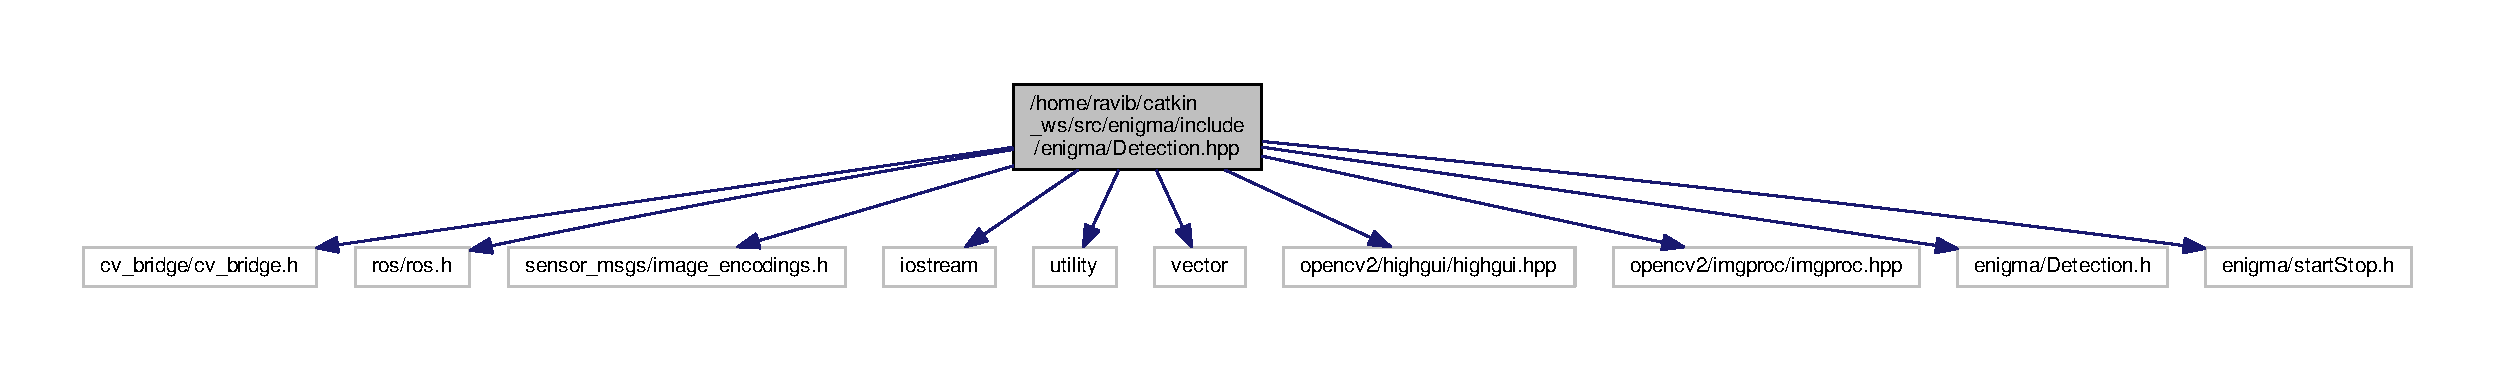
\includegraphics[width=350pt]{_detection_8hpp__incl}
\end{center}
\end{figure}
This graph shows which files directly or indirectly include this file\+:
\nopagebreak
\begin{figure}[H]
\begin{center}
\leavevmode
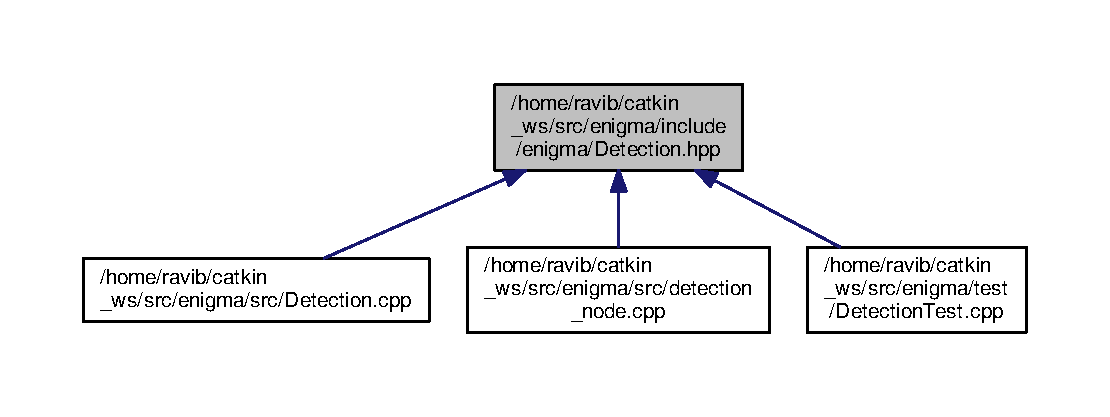
\includegraphics[width=350pt]{_detection_8hpp__dep__incl}
\end{center}
\end{figure}
\subsection*{Classes}
\begin{DoxyCompactItemize}
\item 
class \hyperlink{class_detection}{Detection}
\begin{DoxyCompactList}\small\item\em Class for detection. \end{DoxyCompactList}\end{DoxyCompactItemize}


\subsection{Detailed Description}
Anomaly detection class. 

\begin{DoxyAuthor}{Author}
Ravi Bhadeshiya 
\end{DoxyAuthor}
\begin{DoxyVersion}{Version}
1.\+0 
\end{DoxyVersion}
\begin{DoxyCopyright}{Copyright}
M\+IT License (c) 2017 Ravi Bhadeshiya
\end{DoxyCopyright}
Permission is hereby granted, free of charge, to any person obtaining a copy of this software and associated documentation files (the \char`\"{}\+Software\char`\"{}), to deal in the Software without restriction, including without limitation the rights to use, copy, modify, merge, publish, distribute, sublicense, and/or sell copies of the Software, and to permit persons to whom the Software is furnished to do so, subject to the following conditions\+:

The above copyright notice and this permission notice shall be included in all copies or substantial portions of the Software.

T\+HE S\+O\+F\+T\+W\+A\+RE IS P\+R\+O\+V\+I\+D\+ED \char`\"{}\+A\+S I\+S\char`\"{}, W\+I\+T\+H\+O\+UT W\+A\+R\+R\+A\+N\+TY OF A\+NY K\+I\+ND, E\+X\+P\+R\+E\+SS OR I\+M\+P\+L\+I\+ED, I\+N\+C\+L\+U\+D\+I\+NG B\+UT N\+OT L\+I\+M\+I\+T\+ED TO T\+HE W\+A\+R\+R\+A\+N\+T\+I\+ES OF M\+E\+R\+C\+H\+A\+N\+T\+A\+B\+I\+L\+I\+TY, F\+I\+T\+N\+E\+SS F\+OR A P\+A\+R\+T\+I\+C\+U\+L\+AR P\+U\+R\+P\+O\+SE A\+ND N\+O\+N\+I\+N\+F\+R\+I\+N\+G\+E\+M\+E\+NT. IN NO E\+V\+E\+NT S\+H\+A\+LL T\+HE A\+U\+T\+H\+O\+RS OR C\+O\+P\+Y\+R\+I\+G\+HT H\+O\+L\+D\+E\+RS BE L\+I\+A\+B\+LE F\+OR A\+NY C\+L\+A\+IM, D\+A\+M\+A\+G\+ES OR O\+T\+H\+ER L\+I\+A\+B\+I\+L\+I\+TY, W\+H\+E\+T\+H\+ER IN AN A\+C\+T\+I\+ON OF C\+O\+N\+T\+R\+A\+CT, T\+O\+RT OR O\+T\+H\+E\+R\+W\+I\+SE, A\+R\+I\+S\+I\+NG F\+R\+OM, O\+UT OF OR IN C\+O\+N\+N\+E\+C\+T\+I\+ON W\+I\+TH T\+HE S\+O\+F\+T\+W\+A\+RE OR T\+HE U\+SE OR O\+T\+H\+ER D\+E\+A\+L\+I\+N\+GS IN T\+HE S\+O\+F\+T\+W\+A\+RE. 
\hypertarget{_enigma_8hpp}{}\section{/home/ravib/catkin\+\_\+ws/src/enigma/include/enigma/\+Enigma.hpp File Reference}
\label{_enigma_8hpp}\index{/home/ravib/catkin\+\_\+ws/src/enigma/include/enigma/\+Enigma.\+hpp@{/home/ravib/catkin\+\_\+ws/src/enigma/include/enigma/\+Enigma.\+hpp}}


Class for Security Robot api.  


{\ttfamily \#include $<$enigma/\+Detection.\+h$>$}\newline
{\ttfamily \#include $<$geometry\+\_\+msgs/\+Twist.\+h$>$}\newline
{\ttfamily \#include $<$ros/ros.\+h$>$}\newline
{\ttfamily \#include $<$sensor\+\_\+msgs/\+Laser\+Scan.\+h$>$}\newline
{\ttfamily \#include $<$enigma/change\+Speed.\+h$>$}\newline
{\ttfamily \#include $<$enigma/start\+Stop.\+h$>$}\newline
{\ttfamily \#include $<$cmath$>$}\newline
Include dependency graph for Enigma.\+hpp\+:
\nopagebreak
\begin{figure}[H]
\begin{center}
\leavevmode
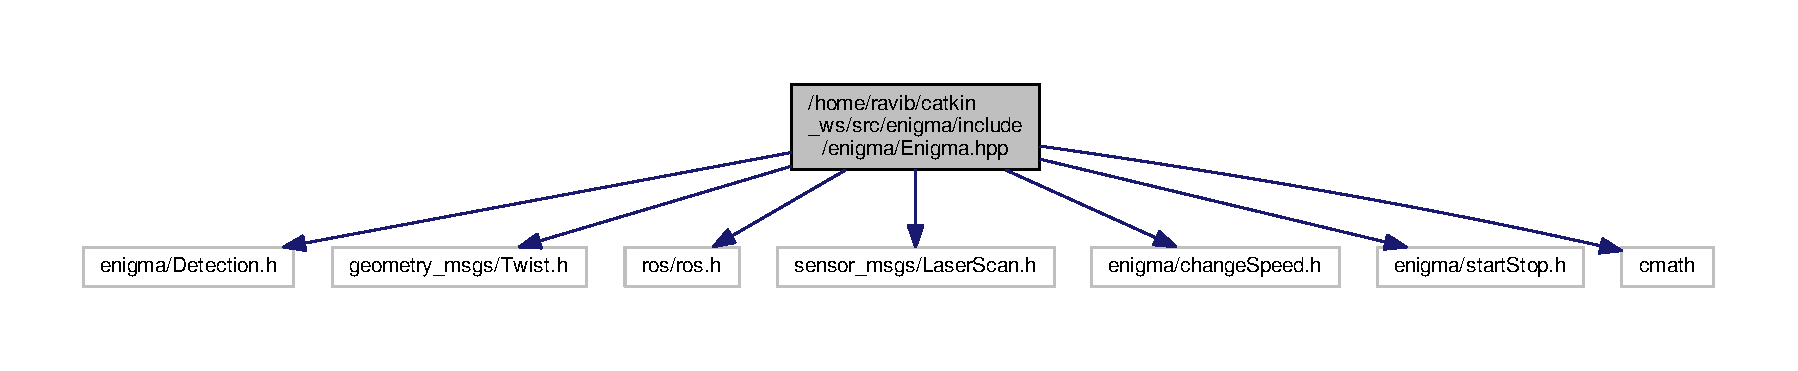
\includegraphics[width=350pt]{_enigma_8hpp__incl}
\end{center}
\end{figure}
This graph shows which files directly or indirectly include this file\+:
\nopagebreak
\begin{figure}[H]
\begin{center}
\leavevmode
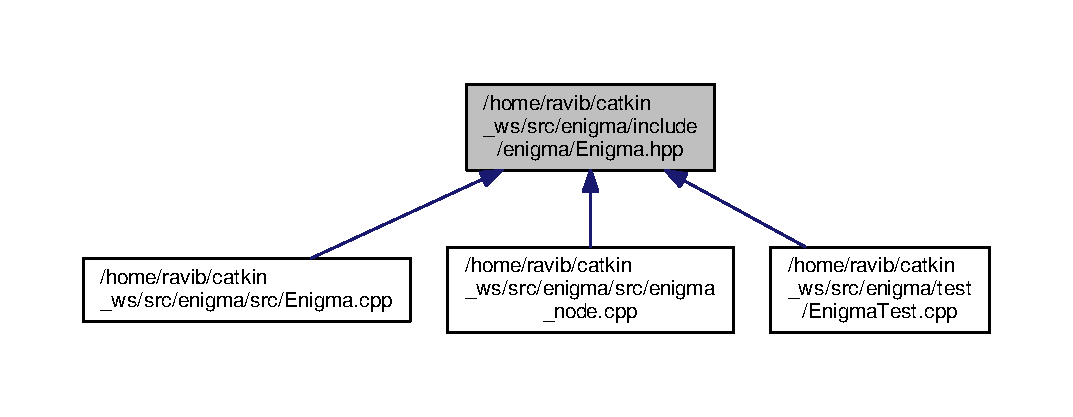
\includegraphics[width=350pt]{_enigma_8hpp__dep__incl}
\end{center}
\end{figure}
\subsection*{Classes}
\begin{DoxyCompactItemize}
\item 
class \hyperlink{class_enigma}{Enigma}
\begin{DoxyCompactList}\small\item\em Class for enigma for robot behavior. \end{DoxyCompactList}\end{DoxyCompactItemize}


\subsection{Detailed Description}
Class for Security Robot api. 

\begin{DoxyAuthor}{Author}
Ravi Bhadeshiya 
\end{DoxyAuthor}
\begin{DoxyVersion}{Version}
1.\+0 
\end{DoxyVersion}
\begin{DoxyCopyright}{Copyright}
M\+IT License (c) 2017 Ravi Bhadeshiya
\end{DoxyCopyright}
Permission is hereby granted, free of charge, to any person obtaining a copy of this software and associated documentation files (the \char`\"{}\+Software\char`\"{}), to deal in the Software without restriction, including without limitation the rights to use, copy, modify, merge, publish, distribute, sublicense, and/or sell copies of the Software, and to permit persons to whom the Software is furnished to do so, subject to the following conditions\+:

The above copyright notice and this permission notice shall be included in all copies or substantial portions of the Software.

T\+HE S\+O\+F\+T\+W\+A\+RE IS P\+R\+O\+V\+I\+D\+ED \char`\"{}\+A\+S I\+S\char`\"{}, W\+I\+T\+H\+O\+UT W\+A\+R\+R\+A\+N\+TY OF A\+NY K\+I\+ND, E\+X\+P\+R\+E\+SS OR I\+M\+P\+L\+I\+ED, I\+N\+C\+L\+U\+D\+I\+NG B\+UT N\+OT L\+I\+M\+I\+T\+ED TO T\+HE W\+A\+R\+R\+A\+N\+T\+I\+ES OF M\+E\+R\+C\+H\+A\+N\+T\+A\+B\+I\+L\+I\+TY, F\+I\+T\+N\+E\+SS F\+OR A P\+A\+R\+T\+I\+C\+U\+L\+AR P\+U\+R\+P\+O\+SE A\+ND N\+O\+N\+I\+N\+F\+R\+I\+N\+G\+E\+M\+E\+NT. IN NO E\+V\+E\+NT S\+H\+A\+LL T\+HE A\+U\+T\+H\+O\+RS OR C\+O\+P\+Y\+R\+I\+G\+HT H\+O\+L\+D\+E\+RS BE L\+I\+A\+B\+LE F\+OR A\+NY C\+L\+A\+IM, D\+A\+M\+A\+G\+ES OR O\+T\+H\+ER L\+I\+A\+B\+I\+L\+I\+TY, W\+H\+E\+T\+H\+ER IN AN A\+C\+T\+I\+ON OF C\+O\+N\+T\+R\+A\+CT, T\+O\+RT OR O\+T\+H\+E\+R\+W\+I\+SE, A\+R\+I\+S\+I\+NG F\+R\+OM, O\+UT OF OR IN C\+O\+N\+N\+E\+C\+T\+I\+ON W\+I\+TH T\+HE S\+O\+F\+T\+W\+A\+RE OR T\+HE U\+SE OR O\+T\+H\+ER D\+E\+A\+L\+I\+N\+GS IN T\+HE S\+O\+F\+T\+W\+A\+RE. 
\hypertarget{_detection_8cpp}{}\section{/home/ravib/catkin\+\_\+ws/src/enigma/src/\+Detection.cpp File Reference}
\label{_detection_8cpp}\index{/home/ravib/catkin\+\_\+ws/src/enigma/src/\+Detection.\+cpp@{/home/ravib/catkin\+\_\+ws/src/enigma/src/\+Detection.\+cpp}}


Anomaly \hyperlink{class_detection}{Detection} Class.  


{\ttfamily \#include \char`\"{}enigma/\+Detection.\+hpp\char`\"{}}\newline
Include dependency graph for Detection.\+cpp\+:
\nopagebreak
\begin{figure}[H]
\begin{center}
\leavevmode
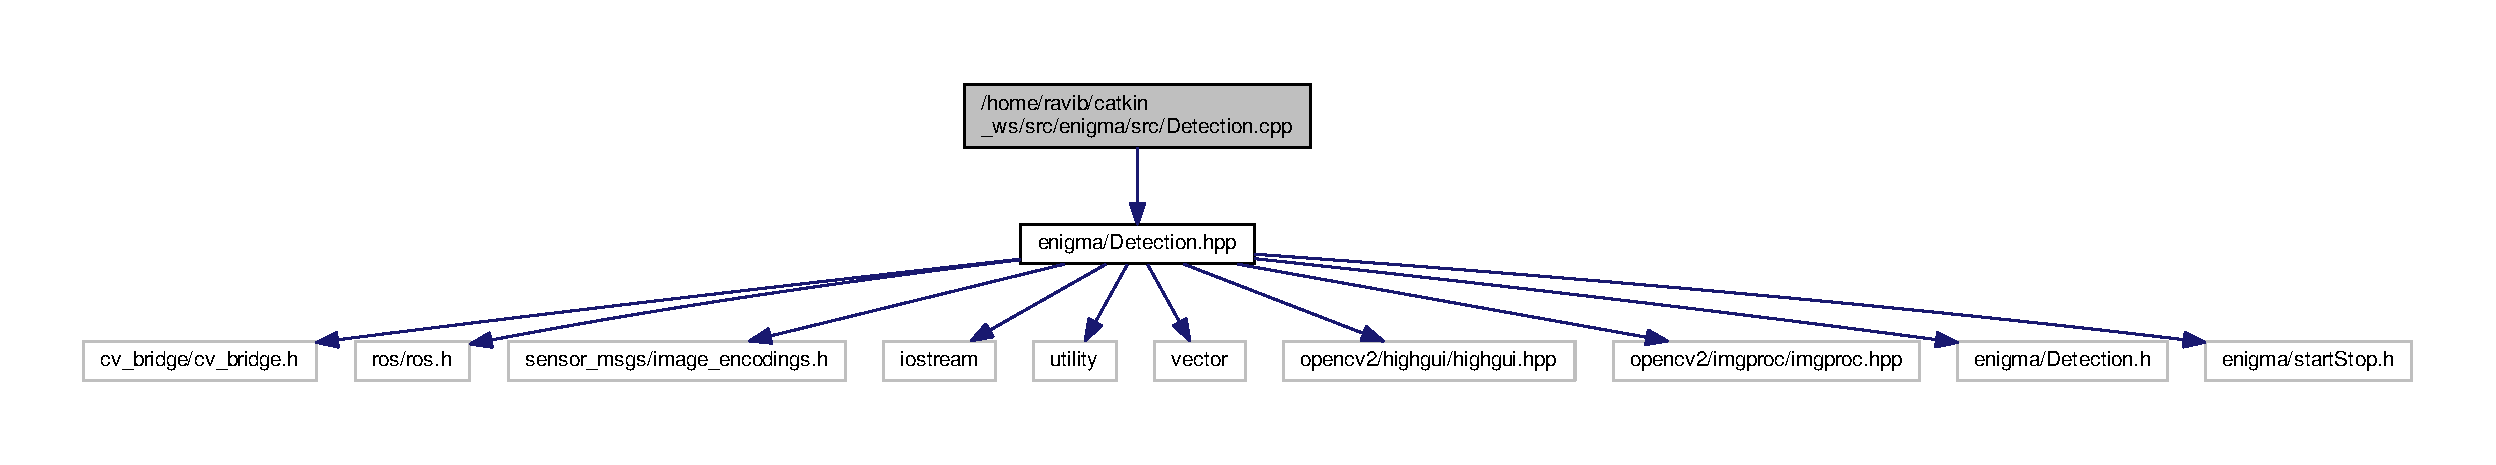
\includegraphics[width=350pt]{_detection_8cpp__incl}
\end{center}
\end{figure}


\subsection{Detailed Description}
Anomaly \hyperlink{class_detection}{Detection} Class. 

\begin{DoxyAuthor}{Author}
Ravi Bhadeshiya 
\end{DoxyAuthor}
\begin{DoxyVersion}{Version}
1.\+0 
\end{DoxyVersion}
\begin{DoxyCopyright}{Copyright}
M\+IT License (c) 2017 Ravi Bhadeshiya
\end{DoxyCopyright}
Permission is hereby granted, free of charge, to any person obtaining a copy of this software and associated documentation files (the \char`\"{}\+Software\char`\"{}), to deal in the Software without restriction, including without limitation the rights to use, copy, modify, merge, publish, distribute, sublicense, and/or sell copies of the Software, and to permit persons to whom the Software is furnished to do so, subject to the following conditions\+:

The above copyright notice and this permission notice shall be included in all copies or substantial portions of the Software.

T\+HE S\+O\+F\+T\+W\+A\+RE IS P\+R\+O\+V\+I\+D\+ED \char`\"{}\+A\+S I\+S\char`\"{}, W\+I\+T\+H\+O\+UT W\+A\+R\+R\+A\+N\+TY OF A\+NY K\+I\+ND, E\+X\+P\+R\+E\+SS OR I\+M\+P\+L\+I\+ED, I\+N\+C\+L\+U\+D\+I\+NG B\+UT N\+OT L\+I\+M\+I\+T\+ED TO T\+HE W\+A\+R\+R\+A\+N\+T\+I\+ES OF M\+E\+R\+C\+H\+A\+N\+T\+A\+B\+I\+L\+I\+TY, F\+I\+T\+N\+E\+SS F\+OR A P\+A\+R\+T\+I\+C\+U\+L\+AR P\+U\+R\+P\+O\+SE A\+ND N\+O\+N\+I\+N\+F\+R\+I\+N\+G\+E\+M\+E\+NT. IN NO E\+V\+E\+NT S\+H\+A\+LL T\+HE A\+U\+T\+H\+O\+RS OR C\+O\+P\+Y\+R\+I\+G\+HT H\+O\+L\+D\+E\+RS BE L\+I\+A\+B\+LE F\+OR A\+NY C\+L\+A\+IM, D\+A\+M\+A\+G\+ES OR O\+T\+H\+ER L\+I\+A\+B\+I\+L\+I\+TY, W\+H\+E\+T\+H\+ER IN AN A\+C\+T\+I\+ON OF C\+O\+N\+T\+R\+A\+CT, T\+O\+RT OR O\+T\+H\+E\+R\+W\+I\+SE, A\+R\+I\+S\+I\+NG F\+R\+OM, O\+UT OF OR IN C\+O\+N\+N\+E\+C\+T\+I\+ON W\+I\+TH T\+HE S\+O\+F\+T\+W\+A\+RE OR T\+HE U\+SE OR O\+T\+H\+ER D\+E\+A\+L\+I\+N\+GS IN T\+HE S\+O\+F\+T\+W\+A\+RE. 
\hypertarget{_enigma_8cpp}{}\section{/home/ravib/catkin\+\_\+ws/src/enigma/src/\+Enigma.cpp File Reference}
\label{_enigma_8cpp}\index{/home/ravib/catkin\+\_\+ws/src/enigma/src/\+Enigma.\+cpp@{/home/ravib/catkin\+\_\+ws/src/enigma/src/\+Enigma.\+cpp}}


Class for Security Robot api.  


{\ttfamily \#include \char`\"{}enigma/\+Enigma.\+hpp\char`\"{}}\newline
Include dependency graph for Enigma.\+cpp\+:
\nopagebreak
\begin{figure}[H]
\begin{center}
\leavevmode
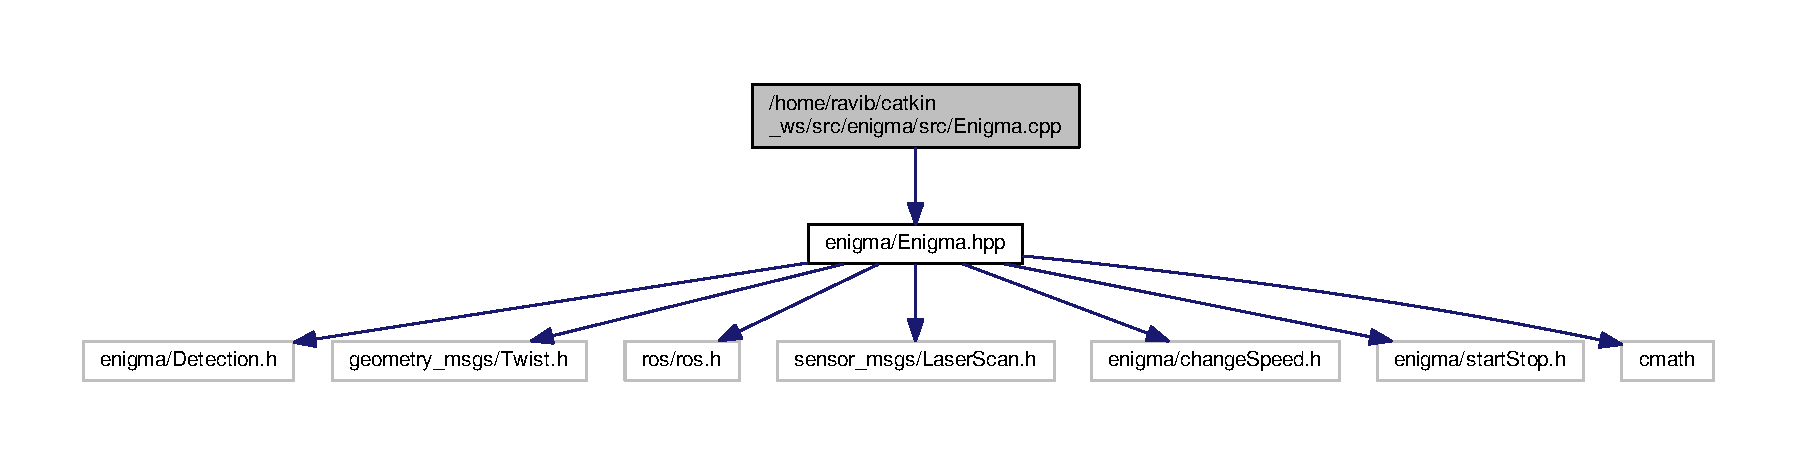
\includegraphics[width=350pt]{_enigma_8cpp__incl}
\end{center}
\end{figure}


\subsection{Detailed Description}
Class for Security Robot api. 

\begin{DoxyAuthor}{Author}
Ravi Bhadeshiya 
\end{DoxyAuthor}
\begin{DoxyVersion}{Version}
1.\+0 
\end{DoxyVersion}
\begin{DoxyCopyright}{Copyright}
M\+IT License (c) 2017 Ravi Bhadeshiya
\end{DoxyCopyright}
Permission is hereby granted, free of charge, to any person obtaining a copy of this software and associated documentation files (the \char`\"{}\+Software\char`\"{}), to deal in the Software without restriction, including without limitation the rights to use, copy, modify, merge, publish, distribute, sublicense, and/or sell copies of the Software, and to permit persons to whom the Software is furnished to do so, subject to the following conditions\+:

The above copyright notice and this permission notice shall be included in all copies or substantial portions of the Software.

T\+HE S\+O\+F\+T\+W\+A\+RE IS P\+R\+O\+V\+I\+D\+ED \char`\"{}\+A\+S I\+S\char`\"{}, W\+I\+T\+H\+O\+UT W\+A\+R\+R\+A\+N\+TY OF A\+NY K\+I\+ND, E\+X\+P\+R\+E\+SS OR I\+M\+P\+L\+I\+ED, I\+N\+C\+L\+U\+D\+I\+NG B\+UT N\+OT L\+I\+M\+I\+T\+ED TO T\+HE W\+A\+R\+R\+A\+N\+T\+I\+ES OF M\+E\+R\+C\+H\+A\+N\+T\+A\+B\+I\+L\+I\+TY, F\+I\+T\+N\+E\+SS F\+OR A P\+A\+R\+T\+I\+C\+U\+L\+AR P\+U\+R\+P\+O\+SE A\+ND N\+O\+N\+I\+N\+F\+R\+I\+N\+G\+E\+M\+E\+NT. IN NO E\+V\+E\+NT S\+H\+A\+LL T\+HE A\+U\+T\+H\+O\+RS OR C\+O\+P\+Y\+R\+I\+G\+HT H\+O\+L\+D\+E\+RS BE L\+I\+A\+B\+LE F\+OR A\+NY C\+L\+A\+IM, D\+A\+M\+A\+G\+ES OR O\+T\+H\+ER L\+I\+A\+B\+I\+L\+I\+TY, W\+H\+E\+T\+H\+ER IN AN A\+C\+T\+I\+ON OF C\+O\+N\+T\+R\+A\+CT, T\+O\+RT OR O\+T\+H\+E\+R\+W\+I\+SE, A\+R\+I\+S\+I\+NG F\+R\+OM, O\+UT OF OR IN C\+O\+N\+N\+E\+C\+T\+I\+ON W\+I\+TH T\+HE S\+O\+F\+T\+W\+A\+RE OR T\+HE U\+SE OR O\+T\+H\+ER D\+E\+A\+L\+I\+N\+GS IN T\+HE S\+O\+F\+T\+W\+A\+RE. 
\hypertarget{enigma__node_8cpp}{}\section{/home/ravib/catkin\+\_\+ws/src/enigma/src/enigma\+\_\+node.cpp File Reference}
\label{enigma__node_8cpp}\index{/home/ravib/catkin\+\_\+ws/src/enigma/src/enigma\+\_\+node.\+cpp@{/home/ravib/catkin\+\_\+ws/src/enigma/src/enigma\+\_\+node.\+cpp}}


The main node for enigma package.  


{\ttfamily \#include \char`\"{}ros/ros.\+h\char`\"{}}\newline
{\ttfamily \#include \char`\"{}std\+\_\+msgs/\+String.\+h\char`\"{}}\newline
{\ttfamily \#include \char`\"{}enigma/\+Enigma.\+hpp\char`\"{}}\newline
Include dependency graph for enigma\+\_\+node.\+cpp\+:
\nopagebreak
\begin{figure}[H]
\begin{center}
\leavevmode
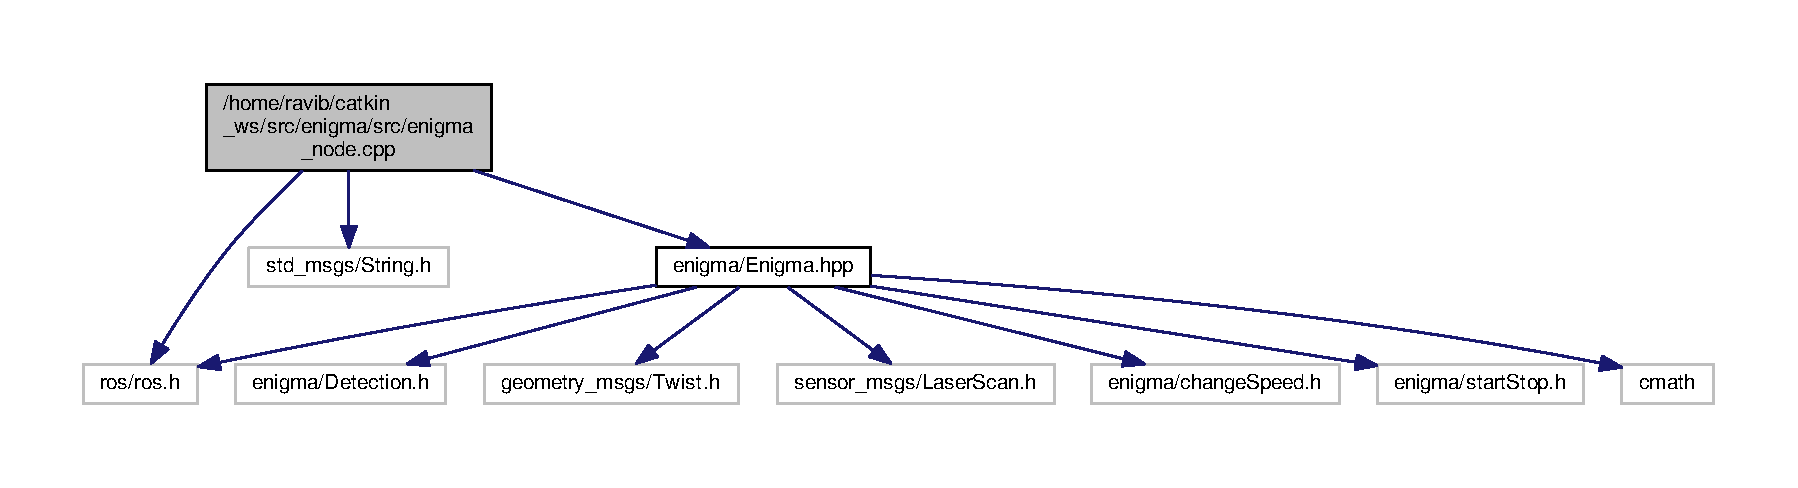
\includegraphics[width=350pt]{enigma__node_8cpp__incl}
\end{center}
\end{figure}
\subsection*{Functions}
\begin{DoxyCompactItemize}
\item 
\mbox{\Hypertarget{enigma__node_8cpp_a3c04138a5bfe5d72780bb7e82a18e627}\label{enigma__node_8cpp_a3c04138a5bfe5d72780bb7e82a18e627}} 
int {\bfseries main} (int argc, char $\ast$$\ast$argv)
\end{DoxyCompactItemize}


\subsection{Detailed Description}
The main node for enigma package. 

\begin{DoxyAuthor}{Author}
Ravi Bhadeshiya 
\end{DoxyAuthor}
\begin{DoxyVersion}{Version}
1.\+0 
\end{DoxyVersion}
\begin{DoxyCopyright}{Copyright}
M\+IT License (c) 2017 Ravi Bhadeshiya
\end{DoxyCopyright}
Permission is hereby granted, free of charge, to any person obtaining a copy of this software and associated documentation files (the \char`\"{}\+Software\char`\"{}), to deal in the Software without restriction, including without limitation the rights to use, copy, modify, merge, publish, distribute, sublicense, and/or sell copies of the Software, and to permit persons to whom the Software is furnished to do so, subject to the following conditions\+:

The above copyright notice and this permission notice shall be included in all copies or substantial portions of the Software.

T\+HE S\+O\+F\+T\+W\+A\+RE IS P\+R\+O\+V\+I\+D\+ED \char`\"{}\+A\+S I\+S\char`\"{}, W\+I\+T\+H\+O\+UT W\+A\+R\+R\+A\+N\+TY OF A\+NY K\+I\+ND, E\+X\+P\+R\+E\+SS OR I\+M\+P\+L\+I\+ED, I\+N\+C\+L\+U\+D\+I\+NG B\+UT N\+OT L\+I\+M\+I\+T\+ED TO T\+HE W\+A\+R\+R\+A\+N\+T\+I\+ES OF M\+E\+R\+C\+H\+A\+N\+T\+A\+B\+I\+L\+I\+TY, F\+I\+T\+N\+E\+SS F\+OR A P\+A\+R\+T\+I\+C\+U\+L\+AR P\+U\+R\+P\+O\+SE A\+ND N\+O\+N\+I\+N\+F\+R\+I\+N\+G\+E\+M\+E\+NT. IN NO E\+V\+E\+NT S\+H\+A\+LL T\+HE A\+U\+T\+H\+O\+RS OR C\+O\+P\+Y\+R\+I\+G\+HT H\+O\+L\+D\+E\+RS BE L\+I\+A\+B\+LE F\+OR A\+NY C\+L\+A\+IM, D\+A\+M\+A\+G\+ES OR O\+T\+H\+ER L\+I\+A\+B\+I\+L\+I\+TY, W\+H\+E\+T\+H\+ER IN AN A\+C\+T\+I\+ON OF C\+O\+N\+T\+R\+A\+CT, T\+O\+RT OR O\+T\+H\+E\+R\+W\+I\+SE, A\+R\+I\+S\+I\+NG F\+R\+OM, O\+UT OF OR IN C\+O\+N\+N\+E\+C\+T\+I\+ON W\+I\+TH T\+HE S\+O\+F\+T\+W\+A\+RE OR T\+HE U\+SE OR O\+T\+H\+ER D\+E\+A\+L\+I\+N\+GS IN T\+HE S\+O\+F\+T\+W\+A\+RE. 
\hypertarget{_detection_test_8cpp}{}\section{/home/ravib/catkin\+\_\+ws/src/enigma/test/\+Detection\+Test.cpp File Reference}
\label{_detection_test_8cpp}\index{/home/ravib/catkin\+\_\+ws/src/enigma/test/\+Detection\+Test.\+cpp@{/home/ravib/catkin\+\_\+ws/src/enigma/test/\+Detection\+Test.\+cpp}}


This file contain all the test cases for \hyperlink{class_detection}{Detection}.  


{\ttfamily \#include $<$gtest/gtest.\+h$>$}\newline
{\ttfamily \#include $<$ros/ros.\+h$>$}\newline
{\ttfamily \#include $<$ros/service\+\_\+client.\+h$>$}\newline
{\ttfamily \#include \char`\"{}enigma/\+Detection.\+h\char`\"{}}\newline
{\ttfamily \#include \char`\"{}enigma/\+Detection.\+hpp\char`\"{}}\newline
{\ttfamily \#include \char`\"{}enigma/start\+Stop.\+h\char`\"{}}\newline
Include dependency graph for Detection\+Test.\+cpp\+:
\nopagebreak
\begin{figure}[H]
\begin{center}
\leavevmode
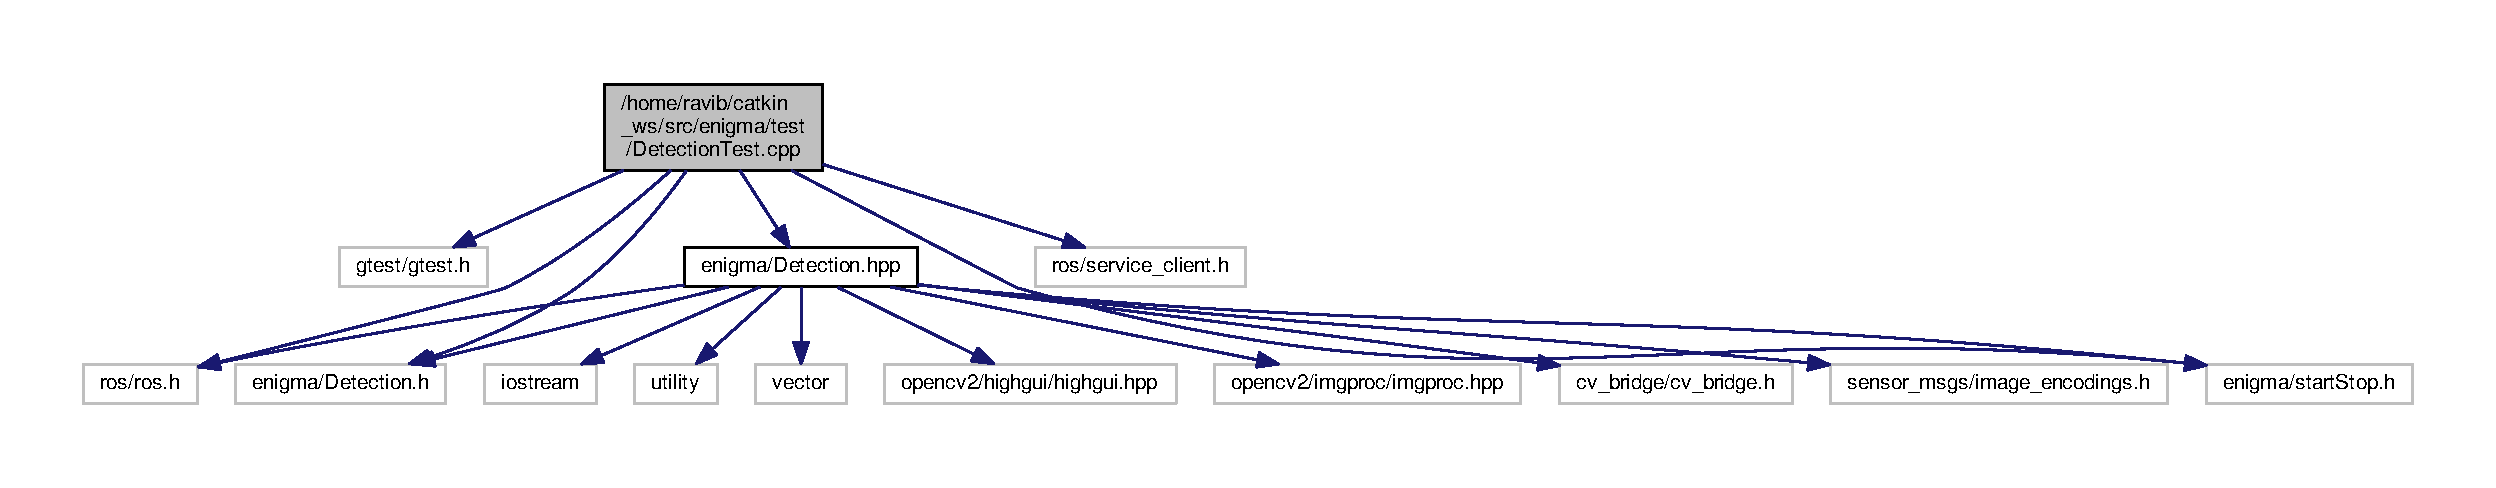
\includegraphics[width=350pt]{_detection_test_8cpp__incl}
\end{center}
\end{figure}
\subsection*{Classes}
\begin{DoxyCompactItemize}
\item 
struct \hyperlink{struct_test_helper}{Test\+Helper}
\begin{DoxyCompactList}\small\item\em Struct for service callback helper. \end{DoxyCompactList}\end{DoxyCompactItemize}
\subsection*{Functions}
\begin{DoxyCompactItemize}
\item 
\mbox{\Hypertarget{_detection_test_8cpp_a5499c7489fa67056e40b3004e2f0d3c6}\label{_detection_test_8cpp_a5499c7489fa67056e40b3004e2f0d3c6}} 
\hyperlink{_detection_test_8cpp_a5499c7489fa67056e40b3004e2f0d3c6}{T\+E\+ST} (T\+E\+S\+T\+\_\+\+D\+E\+T\+E\+C\+T\+I\+ON, Test\+Open\+Cv\+Init)
\begin{DoxyCompactList}\small\item\em To test for \hyperlink{class_detection}{Detection}. \end{DoxyCompactList}\item 
\mbox{\Hypertarget{_detection_test_8cpp_adc3ce3b61992a7723aaa50a3cb5d5680}\label{_detection_test_8cpp_adc3ce3b61992a7723aaa50a3cb5d5680}} 
\hyperlink{_detection_test_8cpp_adc3ce3b61992a7723aaa50a3cb5d5680}{T\+E\+ST} (T\+E\+S\+T\+\_\+\+D\+E\+T\+E\+C\+T\+I\+ON, Test\+Subscriber)
\begin{DoxyCompactList}\small\item\em To test the image subscriber is working properly. \end{DoxyCompactList}\item 
\mbox{\Hypertarget{_detection_test_8cpp_a6476a1b527a30760feba719385c9e625}\label{_detection_test_8cpp_a6476a1b527a30760feba719385c9e625}} 
\hyperlink{_detection_test_8cpp_a6476a1b527a30760feba719385c9e625}{T\+E\+ST} (T\+E\+S\+T\+\_\+\+D\+E\+T\+E\+C\+T\+I\+ON, Test\+Publisher)
\begin{DoxyCompactList}\small\item\em To test the \hyperlink{class_detection}{Detection} publisher. \end{DoxyCompactList}\item 
\mbox{\Hypertarget{_detection_test_8cpp_ab3dd738cc64421b91b9a6661f7eefcc0}\label{_detection_test_8cpp_ab3dd738cc64421b91b9a6661f7eefcc0}} 
\hyperlink{_detection_test_8cpp_ab3dd738cc64421b91b9a6661f7eefcc0}{T\+E\+ST} (T\+E\+S\+T\+\_\+\+D\+E\+T\+E\+C\+T\+I\+ON, Test\+Detection)
\begin{DoxyCompactList}\small\item\em To test the detection method. \end{DoxyCompactList}\item 
\mbox{\Hypertarget{_detection_test_8cpp_ae1f8a2bf15219bfe8e8fb189c9974c60}\label{_detection_test_8cpp_ae1f8a2bf15219bfe8e8fb189c9974c60}} 
\hyperlink{_detection_test_8cpp_ae1f8a2bf15219bfe8e8fb189c9974c60}{T\+E\+ST} (T\+E\+S\+T\+\_\+\+D\+E\+T\+E\+C\+T\+I\+ON, Test\+Switch\+Service)
\begin{DoxyCompactList}\small\item\em Test detection start and stop service. \end{DoxyCompactList}\end{DoxyCompactItemize}


\subsection{Detailed Description}
This file contain all the test cases for \hyperlink{class_detection}{Detection}. 

\begin{DoxyAuthor}{Author}
Ravi Bhadeshiya 
\end{DoxyAuthor}
\begin{DoxyVersion}{Version}
1.\+0 
\end{DoxyVersion}
\begin{DoxyCopyright}{Copyright}
M\+IT License (c) 2017 Ravi Bhadeshiya
\end{DoxyCopyright}
Permission is hereby granted, free of charge, to any person obtaining a copy of this software and associated documentation files (the \char`\"{}\+Software\char`\"{}), to deal in the Software without restriction, including without limitation the rights to use, copy, modify, merge, publish, distribute, sublicense, and/or sell copies of the Software, and to permit persons to whom the Software is furnished to do so, subject to the following conditions\+:

The above copyright notice and this permission notice shall be included in all copies or substantial portions of the Software.

T\+HE S\+O\+F\+T\+W\+A\+RE IS P\+R\+O\+V\+I\+D\+ED \char`\"{}\+A\+S I\+S\char`\"{}, W\+I\+T\+H\+O\+UT W\+A\+R\+R\+A\+N\+TY OF A\+NY K\+I\+ND, E\+X\+P\+R\+E\+SS OR I\+M\+P\+L\+I\+ED, I\+N\+C\+L\+U\+D\+I\+NG B\+UT N\+OT L\+I\+M\+I\+T\+ED TO T\+HE W\+A\+R\+R\+A\+N\+T\+I\+ES OF M\+E\+R\+C\+H\+A\+N\+T\+A\+B\+I\+L\+I\+TY, F\+I\+T\+N\+E\+SS F\+OR A P\+A\+R\+T\+I\+C\+U\+L\+AR P\+U\+R\+P\+O\+SE A\+ND N\+O\+N\+I\+N\+F\+R\+I\+N\+G\+E\+M\+E\+NT. IN NO E\+V\+E\+NT S\+H\+A\+LL T\+HE A\+U\+T\+H\+O\+RS OR C\+O\+P\+Y\+R\+I\+G\+HT H\+O\+L\+D\+E\+RS BE L\+I\+A\+B\+LE F\+OR A\+NY C\+L\+A\+IM, D\+A\+M\+A\+G\+ES OR O\+T\+H\+ER L\+I\+A\+B\+I\+L\+I\+TY, W\+H\+E\+T\+H\+ER IN AN A\+C\+T\+I\+ON OF C\+O\+N\+T\+R\+A\+CT, T\+O\+RT OR O\+T\+H\+E\+R\+W\+I\+SE, A\+R\+I\+S\+I\+NG F\+R\+OM, O\+UT OF OR IN C\+O\+N\+N\+E\+C\+T\+I\+ON W\+I\+TH T\+HE S\+O\+F\+T\+W\+A\+RE OR T\+HE U\+SE OR O\+T\+H\+ER D\+E\+A\+L\+I\+N\+GS IN T\+HE S\+O\+F\+T\+W\+A\+RE. 
\hypertarget{enigma__test__node_8cpp}{}\section{/home/ravib/catkin\+\_\+ws/src/enigma/test/enigma\+\_\+test\+\_\+node.cpp File Reference}
\label{enigma__test__node_8cpp}\index{/home/ravib/catkin\+\_\+ws/src/enigma/test/enigma\+\_\+test\+\_\+node.\+cpp@{/home/ravib/catkin\+\_\+ws/src/enigma/test/enigma\+\_\+test\+\_\+node.\+cpp}}


To test enigma package.  


{\ttfamily \#include $<$gtest/gtest.\+h$>$}\newline
{\ttfamily \#include $<$ros/ros.\+h$>$}\newline
Include dependency graph for enigma\+\_\+test\+\_\+node.\+cpp\+:
\nopagebreak
\begin{figure}[H]
\begin{center}
\leavevmode
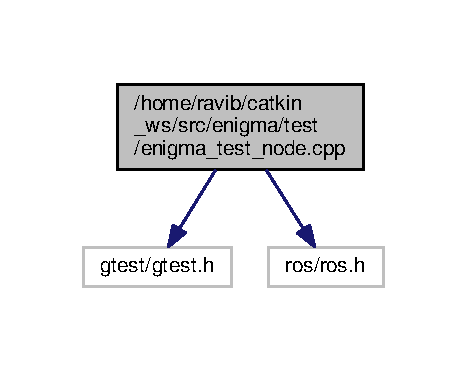
\includegraphics[width=224pt]{enigma__test__node_8cpp__incl}
\end{center}
\end{figure}
\subsection*{Functions}
\begin{DoxyCompactItemize}
\item 
int \hyperlink{enigma__test__node_8cpp_a3c04138a5bfe5d72780bb7e82a18e627}{main} (int argc, char $\ast$$\ast$argv)
\begin{DoxyCompactList}\small\item\em Main function for testing. \end{DoxyCompactList}\end{DoxyCompactItemize}


\subsection{Detailed Description}
To test enigma package. 

\begin{DoxyAuthor}{Author}
Ravi Bhadeshiya 
\end{DoxyAuthor}
\begin{DoxyVersion}{Version}
1.\+0 
\end{DoxyVersion}
\begin{DoxyCopyright}{Copyright}
M\+IT License (c) 2017 Ravi Bhadeshiya
\end{DoxyCopyright}
Permission is hereby granted, free of charge, to any person obtaining a copy of this software and associated documentation files (the \char`\"{}\+Software\char`\"{}), to deal in the Software without restriction, including without limitation the rights to use, copy, modify, merge, publish, distribute, sublicense, and/or sell copies of the Software, and to permit persons to whom the Software is furnished to do so, subject to the following conditions\+:

The above copyright notice and this permission notice shall be included in all copies or substantial portions of the Software.

T\+HE S\+O\+F\+T\+W\+A\+RE IS P\+R\+O\+V\+I\+D\+ED \char`\"{}\+A\+S I\+S\char`\"{}, W\+I\+T\+H\+O\+UT W\+A\+R\+R\+A\+N\+TY OF A\+NY K\+I\+ND, E\+X\+P\+R\+E\+SS OR I\+M\+P\+L\+I\+ED, I\+N\+C\+L\+U\+D\+I\+NG B\+UT N\+OT L\+I\+M\+I\+T\+ED TO T\+HE W\+A\+R\+R\+A\+N\+T\+I\+ES OF M\+E\+R\+C\+H\+A\+N\+T\+A\+B\+I\+L\+I\+TY, F\+I\+T\+N\+E\+SS F\+OR A P\+A\+R\+T\+I\+C\+U\+L\+AR P\+U\+R\+P\+O\+SE A\+ND N\+O\+N\+I\+N\+F\+R\+I\+N\+G\+E\+M\+E\+NT. IN NO E\+V\+E\+NT S\+H\+A\+LL T\+HE A\+U\+T\+H\+O\+RS OR C\+O\+P\+Y\+R\+I\+G\+HT H\+O\+L\+D\+E\+RS BE L\+I\+A\+B\+LE F\+OR A\+NY C\+L\+A\+IM, D\+A\+M\+A\+G\+ES OR O\+T\+H\+ER L\+I\+A\+B\+I\+L\+I\+TY, W\+H\+E\+T\+H\+ER IN AN A\+C\+T\+I\+ON OF C\+O\+N\+T\+R\+A\+CT, T\+O\+RT OR O\+T\+H\+E\+R\+W\+I\+SE, A\+R\+I\+S\+I\+NG F\+R\+OM, O\+UT OF OR IN C\+O\+N\+N\+E\+C\+T\+I\+ON W\+I\+TH T\+HE S\+O\+F\+T\+W\+A\+RE OR T\+HE U\+SE OR O\+T\+H\+ER D\+E\+A\+L\+I\+N\+GS IN T\+HE S\+O\+F\+T\+W\+A\+RE. 

\subsection{Function Documentation}
\mbox{\Hypertarget{enigma__test__node_8cpp_a3c04138a5bfe5d72780bb7e82a18e627}\label{enigma__test__node_8cpp_a3c04138a5bfe5d72780bb7e82a18e627}} 
\index{enigma\+\_\+test\+\_\+node.\+cpp@{enigma\+\_\+test\+\_\+node.\+cpp}!main@{main}}
\index{main@{main}!enigma\+\_\+test\+\_\+node.\+cpp@{enigma\+\_\+test\+\_\+node.\+cpp}}
\subsubsection{\texorpdfstring{main()}{main()}}
{\footnotesize\ttfamily int main (\begin{DoxyParamCaption}\item[{int}]{argc,  }\item[{char $\ast$$\ast$}]{argv }\end{DoxyParamCaption})}



Main function for testing. 


\begin{DoxyParams}[1]{Parameters}
\mbox{\tt in}  & {\em argc} & The argc as int \\
\hline
 & {\em argv} & The argv as char array\\
\hline
\end{DoxyParams}
\begin{DoxyReturn}{Returns}
0 if everything passed 
\end{DoxyReturn}


Definition at line 38 of file enigma\+\_\+test\+\_\+node.\+cpp.


\hypertarget{_enigma_test_8cpp}{}\section{/home/ravib/catkin\+\_\+ws/src/enigma/test/\+Enigma\+Test.cpp File Reference}
\label{_enigma_test_8cpp}\index{/home/ravib/catkin\+\_\+ws/src/enigma/test/\+Enigma\+Test.\+cpp@{/home/ravib/catkin\+\_\+ws/src/enigma/test/\+Enigma\+Test.\+cpp}}


This file contain all the test cases for \hyperlink{class_enigma}{Enigma}.  


{\ttfamily \#include $<$gtest/gtest.\+h$>$}\newline
{\ttfamily \#include $<$ros/ros.\+h$>$}\newline
{\ttfamily \#include $<$memory$>$}\newline
{\ttfamily \#include \char`\"{}enigma/\+Enigma.\+hpp\char`\"{}}\newline
{\ttfamily \#include \char`\"{}enigma/change\+Speed.\+h\char`\"{}}\newline
{\ttfamily \#include \char`\"{}enigma/start\+Stop.\+h\char`\"{}}\newline
Include dependency graph for Enigma\+Test.\+cpp\+:
\nopagebreak
\begin{figure}[H]
\begin{center}
\leavevmode
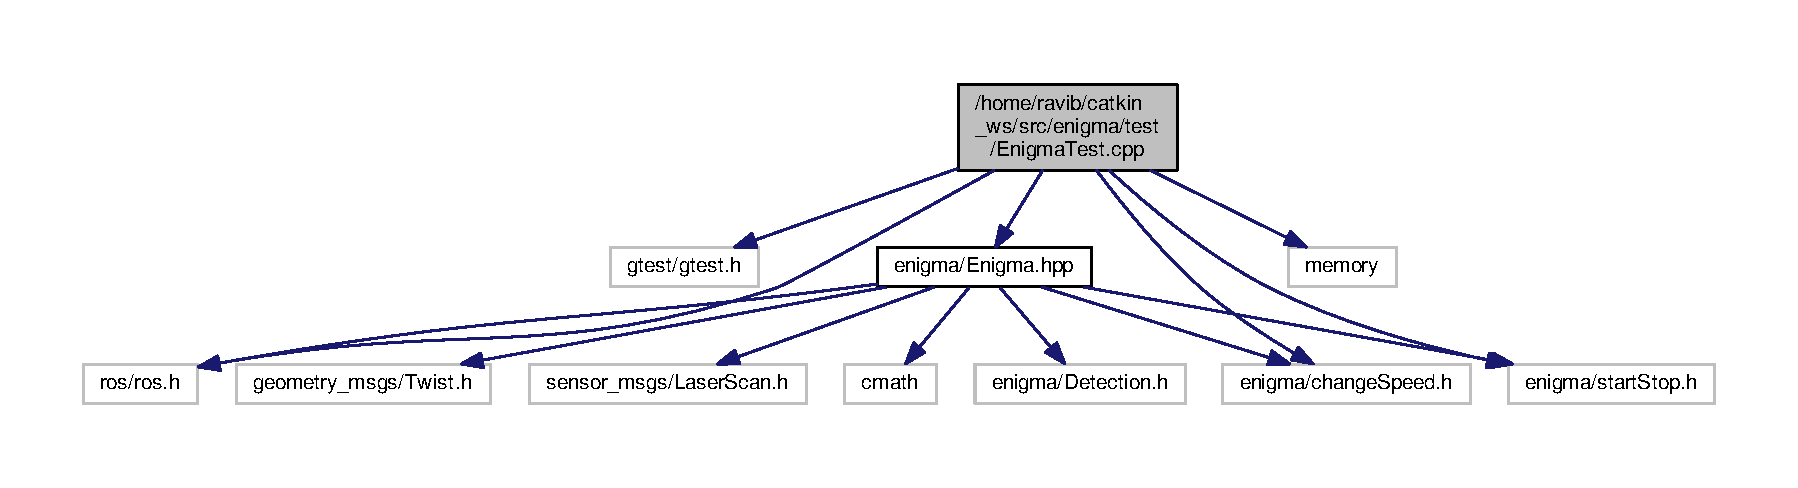
\includegraphics[width=350pt]{_enigma_test_8cpp__incl}
\end{center}
\end{figure}
\subsection*{Functions}
\begin{DoxyCompactItemize}
\item 
\mbox{\Hypertarget{_enigma_test_8cpp_a43e8f801cf4e130572b38a7118a527ef}\label{_enigma_test_8cpp_a43e8f801cf4e130572b38a7118a527ef}} 
\hyperlink{_enigma_test_8cpp_a43e8f801cf4e130572b38a7118a527ef}{T\+E\+ST} (T\+E\+S\+T\+\_\+\+Enigma, Test\+Init)
\begin{DoxyCompactList}\small\item\em To test \hyperlink{class_enigma}{Enigma}. \end{DoxyCompactList}\item 
\mbox{\Hypertarget{_enigma_test_8cpp_a28309cb321c1f9b5cd02cc759d7c80f5}\label{_enigma_test_8cpp_a28309cb321c1f9b5cd02cc759d7c80f5}} 
\hyperlink{_enigma_test_8cpp_a28309cb321c1f9b5cd02cc759d7c80f5}{T\+E\+ST} (T\+E\+S\+T\+\_\+\+Enigma, no\+Obst)
\begin{DoxyCompactList}\small\item\em Test behavior without obst. \end{DoxyCompactList}\item 
\mbox{\Hypertarget{_enigma_test_8cpp_aeafda756655a02c379ca88b2fcb15600}\label{_enigma_test_8cpp_aeafda756655a02c379ca88b2fcb15600}} 
\hyperlink{_enigma_test_8cpp_aeafda756655a02c379ca88b2fcb15600}{T\+E\+ST} (T\+E\+S\+T\+\_\+\+Enigma, obst)
\begin{DoxyCompactList}\small\item\em Test behavior with obst. \end{DoxyCompactList}\item 
\mbox{\Hypertarget{_enigma_test_8cpp_a1771dc138f6934213b11428bc041f338}\label{_enigma_test_8cpp_a1771dc138f6934213b11428bc041f338}} 
\hyperlink{_enigma_test_8cpp_a1771dc138f6934213b11428bc041f338}{T\+E\+ST} (T\+E\+S\+T\+\_\+\+Enigma, detecion\+CB)
\begin{DoxyCompactList}\small\item\em Test detection callback. \end{DoxyCompactList}\item 
\mbox{\Hypertarget{_enigma_test_8cpp_aec60224dcd922e1535861ec34a2156f0}\label{_enigma_test_8cpp_aec60224dcd922e1535861ec34a2156f0}} 
\hyperlink{_enigma_test_8cpp_aec60224dcd922e1535861ec34a2156f0}{T\+E\+ST} (T\+E\+S\+T\+\_\+\+Enigma, Test\+Switch\+Service)
\begin{DoxyCompactList}\small\item\em Test robot start and stop service. \end{DoxyCompactList}\item 
\mbox{\Hypertarget{_enigma_test_8cpp_a56a403dd40c72c52cba0fe63a05b08fa}\label{_enigma_test_8cpp_a56a403dd40c72c52cba0fe63a05b08fa}} 
\hyperlink{_enigma_test_8cpp_a56a403dd40c72c52cba0fe63a05b08fa}{T\+E\+ST} (T\+E\+S\+T\+\_\+\+Enigma, Test\+Speed\+Service)
\begin{DoxyCompactList}\small\item\em Test robot speed change service. \end{DoxyCompactList}\end{DoxyCompactItemize}


\subsection{Detailed Description}
This file contain all the test cases for \hyperlink{class_enigma}{Enigma}. 

\begin{DoxyAuthor}{Author}
Ravi Bhadeshiya 
\end{DoxyAuthor}
\begin{DoxyVersion}{Version}
1.\+0 
\end{DoxyVersion}
\begin{DoxyCopyright}{Copyright}
M\+IT License (c) 2017 Ravi Bhadeshiya
\end{DoxyCopyright}
Permission is hereby granted, free of charge, to any person obtaining a copy of this software and associated documentation files (the \char`\"{}\+Software\char`\"{}), to deal in the Software without restriction, including without limitation the rights to use, copy, modify, merge, publish, distribute, sublicense, and/or sell copies of the Software, and to permit persons to whom the Software is furnished to do so, subject to the following conditions\+:

The above copyright notice and this permission notice shall be included in all copies or substantial portions of the Software.

T\+HE S\+O\+F\+T\+W\+A\+RE IS P\+R\+O\+V\+I\+D\+ED \char`\"{}\+A\+S I\+S\char`\"{}, W\+I\+T\+H\+O\+UT W\+A\+R\+R\+A\+N\+TY OF A\+NY K\+I\+ND, E\+X\+P\+R\+E\+SS OR I\+M\+P\+L\+I\+ED, I\+N\+C\+L\+U\+D\+I\+NG B\+UT N\+OT L\+I\+M\+I\+T\+ED TO T\+HE W\+A\+R\+R\+A\+N\+T\+I\+ES OF M\+E\+R\+C\+H\+A\+N\+T\+A\+B\+I\+L\+I\+TY, F\+I\+T\+N\+E\+SS F\+OR A P\+A\+R\+T\+I\+C\+U\+L\+AR P\+U\+R\+P\+O\+SE A\+ND N\+O\+N\+I\+N\+F\+R\+I\+N\+G\+E\+M\+E\+NT. IN NO E\+V\+E\+NT S\+H\+A\+LL T\+HE A\+U\+T\+H\+O\+RS OR C\+O\+P\+Y\+R\+I\+G\+HT H\+O\+L\+D\+E\+RS BE L\+I\+A\+B\+LE F\+OR A\+NY C\+L\+A\+IM, D\+A\+M\+A\+G\+ES OR O\+T\+H\+ER L\+I\+A\+B\+I\+L\+I\+TY, W\+H\+E\+T\+H\+ER IN AN A\+C\+T\+I\+ON OF C\+O\+N\+T\+R\+A\+CT, T\+O\+RT OR O\+T\+H\+E\+R\+W\+I\+SE, A\+R\+I\+S\+I\+NG F\+R\+OM, O\+UT OF OR IN C\+O\+N\+N\+E\+C\+T\+I\+ON W\+I\+TH T\+HE S\+O\+F\+T\+W\+A\+RE OR T\+HE U\+SE OR O\+T\+H\+ER D\+E\+A\+L\+I\+N\+GS IN T\+HE S\+O\+F\+T\+W\+A\+RE. 
%--- End generated contents ---

% Index
\backmatter
\newpage
\phantomsection
\clearemptydoublepage
\addcontentsline{toc}{chapter}{Index}
\printindex

\end{document}
